\documentclass[11pt]{amsart}
\usepackage{float}
\usepackage{amsfonts, amstext, amsmath, amsthm, amscd, amssymb, upgreek}
\usepackage{bbm}
\usepackage{graphicx, color,  subfigure, wrapfig, overpic}
\usepackage{fullpage}
%\usepackage[all,cmtip]{xy} 
%\usepackage{mystyle}

%%%%%%%%%%%%%%%%%% Tikz %%%%%%%%%
\usepackage{tikz}
\usetikzlibrary{shapes.geometric, arrows}
\usetikzlibrary{shapes.multipart} %% for multiple lines in node (must have align=center)
\usetikzlibrary{calc}
\usetikzlibrary{scopes}
\usetikzlibrary{math}
\usetikzlibrary{decorations.markings,decorations.pathreplacing}
\usetikzlibrary{fadings}
\usepackage{tikz-cd}

\setlength{\textwidth}{\paperwidth}
\addtolength{\textwidth}{-2in}
\setlength{\textheight}{\paperheight}
\addtolength{\textheight}{-2in}
\calclayout

\tikzset{
every picture/.style={line width=0.8pt, >=stealth,
                       baseline=-3pt,label distance=-3pt},
%%%%%%%%%%  Node styles
emptynode/.style={circle,minimum size=0pt, inner sep=0pt, outer
sep=0},
dotnode/.style={fill=black,circle,minimum size=2.5pt, inner sep=1pt, outer
sep=0},
small_dotnode/.style={fill=black,circle,minimum size=2pt, inner sep=0pt, outer
sep=0},
morphism/.style={fill=white,circle,draw,thin, inner sep=1pt, minimum size=15pt,
                 scale=0.8},
small_morphism/.style={fill=white,circle,draw,thin,inner sep=1pt,
                       minimum size=10pt, scale=0.8},
ellipse_morphism/.style args={#1}{fill=white,circle,draw,thin,inner sep=1pt,
                       minimum size=5pt, scale=0.8,
												ellipse, draw, rotate=#1},
%note that ellipse stretches based on the text inside, so put \;\;\; in label
coupon/.style={draw,thin, inner sep=1pt, minimum size=18pt,scale=0.8},
semi_morphism/.style args={#1,#2}{
                  fill=white,semicircle,draw,thin, inner sep=1pt, scale=0.8,
                  shape border rotate=#1,
                  label={#1-90:#2}},
%%can only rotate semi_morphisms by right angles tho
%%%% different line styles:
regular/.style={densely dashed}, %% for the regular color, i.e. sum d_i
edge/.style={very thick, draw=green, text=black},
overline/.style={preaction={draw,line width=2mm,white,-}},
thin_overline/.style={preaction={draw,line width=#1 mm,white,-}},
thin_overline/.default=2,
thick_overline/.style={preaction={draw,line width=3mm,white,-}},
really_thick/.style={line width=3mm, gray},
%drinfeld center/.style={>=stealth,green!60!black, double
%distance=1pt,text=black},
boundary/.style={thick,  draw=blue, text=black},
%arrow_decoration={markings, mark=at position 0.5 with {\arrow{>}}}
ribbon/.style={line width=1.5mm, postaction={draw,line width=1mm,white}},
ribbon_u/.style args={#1,#2}{line width=#1mm, postaction={draw,line width=#2mm,white}},
%use line width=0.4pt for thin lines to point to things
%%%%%%% Fill styles %%%%%%%%%%%%%%%
cell/.style={fill=black!10},
subgraph/.style={fill=black!30},
%%%%%%% Mid-path arrows
midarrow/.style={postaction={decorate},
                 decoration={
                    markings,% switch on markings
                    mark=at position #1 with {\arrow{>}},
                 }},
midarrow/.default=0.5,
%%%%% Mid-path arrow but reverse
midarrow_rev/.style={postaction={decorate},
                 decoration={
                    markings,% switch on markings
                    mark=at position #1 with {\arrow{<}},
                 }},
midarrow_rev/.default=0.5,
%%%%% for the flowchart; need align=center to allow multiline in node
block/.style={rectangle, rounded corners, text centered, draw=black, align=center}
}

%% style for flow chart blocks
\tikzstyle{block} = [rectangle, rounded corners, text centered, draw=black, align=center]

%% for shading with gradients
\tikzfading[name=fade inside, inner color=transparent!80, outer
color=transparent!10]

%% colors
\definecolor{light-gray}{gray}{0.9}
\definecolor{med-gray}{gray}{0.6}


%%%end tikz stuff %%%%%%%%%%%%%%%%%%%%%%%%%%%%%%%%%%%%%%%%%%%%%%%%%%%%%%%%%%%%


\newcommand{\thmref}[1]{Theorem \ref{#1}}
\newcommand{\prpref}[1]{Proposition \ref{#1}}
\newcommand{\lemref}[1]{Lemma \ref{#1}}
\newcommand{\defref}[1]{Definition \ref{#1}}
\newcommand{\figref}[1]{Figure \ref{#1}}
\newcommand{\secref}[1]{Section \ref{#1}}
\newcommand{\remref}[1]{Remark \ref{#1}}
\newcommand{\eqnref}[1]{(\ref{#1})}
%\newcommand{\ref}[1]{Figure \ref{#1}}
\newcommand{\comment}[1]{}
\newcommand{\inv}{{-1}} % annoying to type {-1} when taking inverse


\textwidth 6.07in 
\textheight 8.6in 
\oddsidemargin 0.18in
\evensidemargin 0.18in
% \topmargin -0.07in
 
%%  If the following line is uncommented, we see the labels of theorems, figures, etc. in the margins.
% \usepackage[notref,notcite]{showkeys}
\setlength{\marginparwidth}{0.8in}
\let\oldmarginpar\marginpar
\renewcommand\marginpar[1]{\oldmarginpar[\raggedleft\footnotesize #1]%
{\raggedright\footnotesize #1}}

%This command stops the Math Review numbers appearing in the references! 
\AtBeginDocument{
   \def\MR#1{}
}
\newcommand{\Sp}{{S}}
\newcommand{\C}{\mathbb{C}}
\newcommand{\R}{\mathbb{R}}
\newcommand{\Q}{\mathbb{Q}}
\newcommand{\Z}{\mathbb{Z}}
\newcommand{\N}{\mathbb{N}}
\newcommand{\CC}{\mathbb{C}}
\newcommand{\RR}{\mathbb{R}}
\newcommand{\HH}{\mathbb{H}}
\newcommand{\ZZ}{\mathbb{Z}}
\newcommand{\bfloor}[1]{\left\lfloor #1\right\rfloor}
\renewcommand{\P}{\mathcal P}
\newcommand{\A}{\mathcal A}
\newcommand{\W}{\mathcal W}
\newcommand{\vol}{{\rm vol}}
\newcommand{\cut}{{\backslash \backslash}}
\newcommand{\bdy}{\partial}
\newcommand{\voct}{{v_{\rm oct}}}
\newcommand{\vtet}{{v_{\rm tet}}}
\renewcommand{\L}{\mathcal L}
\newcommand{\cp}{\mathcal{C}}
\newcommand{\toF}{{\overset{F}{\longrightarrow}}}
\newcommand{\K}{\upkappa}

\def\co{\colon\thinspace}


\newcommand{\torus}{{\mathbb{T}^2}}
\newcommand{\sT}{{\mathcal{T}}}
\newcommand{\cD}{{\mathcal{D}}}
\newcommand{\cL}{{\mathcal{L}}}



\newcommand{\RRR}{{\underline{\mathfrak{R}}}}
\newcommand{\QQQ}{{\underline{\mathfrak{Q}}}}
\newcommand{\CCC}{{\underline{\mathfrak{C}}}}
\newcommand{\PPP}{{\underline{\mathbf{\Phi}}}}
\newcommand{\TTT}{{\underline{\mathbf{\Theta}}}}
\newcommand{\LLL}{{\underline{\mathfrak{L}}}}

\newcommand{\cev}[1]{\overset{\leftarrow}{#1}}

\newcommand{\del}{\partial}
\newcommand{\ddd}[1]{{\frac{\del}{\del #1}}}
\newcommand{\vphi}{\varphi}
\newcommand{\veps}{\varepsilon}
\newcommand{\llong}{{\text{long}}}
\newcommand{\Span}{{\text{span}}}
\newcommand{\Pol}{{\text{Pol}}}
\newcommand{\toruscomp}[1]{{\torus \times I - #1}}

\theoremstyle{plain}
\newtheorem{theorem}{Theorem}[section]
\newtheorem{corollary}[theorem]{Corollary}
\newtheorem{lemma}[theorem]{Lemma}
\newtheorem{prop}[theorem]{Proposition}
\newtheorem{claim}[theorem]{Claim}
\newtheorem{conjecture}[theorem]{Conjecture}
\newtheorem{example}[theorem]{Example}
\newtheorem{convention}[theorem]{Convention}

\newtheorem*{namedtheorem}{\theoremname}
\newcommand{\theoremname}{testing}
\newenvironment{named}[1]{\renewcommand{\theoremname}{#1}\begin{namedtheorem}}{\end{namedtheorem}}
\theoremstyle{definition}
\newtheorem{define}[theorem]{Definition}
\newtheorem{definition}[theorem]{Definition}
\newtheorem{question}[theorem]{Question}
\newtheorem{remark}[theorem]{Remark}

\newcommand{\cm}{,\linebreak[1]}


\title{Hyperbolicity of Augmented Links in the Thickened Torus}


\author[Alice Kwon and Ying Hong Tham]{Alice Kwon and Ying Hong Tham}


\begin{document}
\maketitle



%%% \comment{

\begin{abstract}
For a hyperbolic link $K$ in the thickened torus,
we show there is a decomposition of the complement of a link $L$,
obtained from augmenting $K$, into torihedra. We further decompose 
the torihedra into angled pyramids and finally angled tetrahedra.
These fit into an angled structure on a triangulation of the link complement,
and thus by \cite{Casson-Rivin}, this shows
that $L$ is hyperbolic.  
\end{abstract}


\section{Introduction}
\label{s:intro}

Given a twist-reduced diagram of a link $K$, \emph{augmenting} is a process in
which an unknotted circle component (augmentation) is added to one or more twist
regions (a single crossing or a maximal string of bigons) of $K$.
%%By a standard argument using a Dehn twist
%%on the complement of the crossing circle,
%%the added circle component allows us to remove full twists
%%(i.e. pairs of bigons)
%%at the twist region of $K$
%%while keeping the link complement the same.
%%If the twist region has an odd number of crossings,
%%then all but one crossing is removed,
%%whereas if the twist region has an even number of crossings,
%%then all are removed.
%We can remove full twists by a standard argument using a Dehn twist 
%on the complement of the crossing circle.
The newly obtained link is called an 
\emph{augmented link} and the newly obtained diagram is called an 
\emph{augmented link diagram}. See Figure
\ref{fig:Augmentations}. 


Adams showed in \cite{CA} that given a hyperbolic alternating link $K$ in
$\Sp^3$ the link $L$ obtained by augmenting $K$ is hyperbolic. In this paper we
investigate if this statement holds for links in the thickened torus i.e. if $L$
is a link obtained from augmenting a hyperbolic alternating link $K$ in the
thickened torus. We define augmenting similarly for links in the thickened torus
with their associated link diagram on $\torus \times \{0\}.$ 


Menasco \cite{Menasco} showed that there are decompositions
of the complements of alternating links in $\Sp^3$
into two topological polyhedra,
a top polyhedron and a bottom polyhedron.
For alternating links $K$ in the thickened torus,
Champanerkar, Kofman and Purcell \cite{CKP2}
showed that there is a decomposition of the
complement of $K$ into objects called torihedra, which we think of as
counterparts to Menasco's decomposition % of links in $\Sp^3$ into polyhedra,
for links in the thickened torus;
just like Menasco's decomposition, one obtains a top and a bottom torihedron.


In \secref{s:auglinks} we show that for augmented
links in the thickened torus (not necessarily fully augmented),
one can also obtain a decomposition of the
complement into a top and bottom torihedron.
In \secref{s:hyperbolicity}, we prove that
many augmented alternating links in the thickened torus are hyperbolic.


We point out that \cite{kwon2020fully}, the first author
proved that \emph{fully} augmented links in the thickened torus
are hyperbolic, so this paper can be seen as a generalization
of that work.


While revising this paper, we learned that \cite{adams2021generalized}
proves a generalization of our work here,
showing hyperbolicity of generalized augmented links
in an arbitrary thickened surface.
We note that our approach, based on angle structures,
is different from theirs, which is based on topological arguments.



\begin{figure}
\centering  
\begin{tabular}{cc}
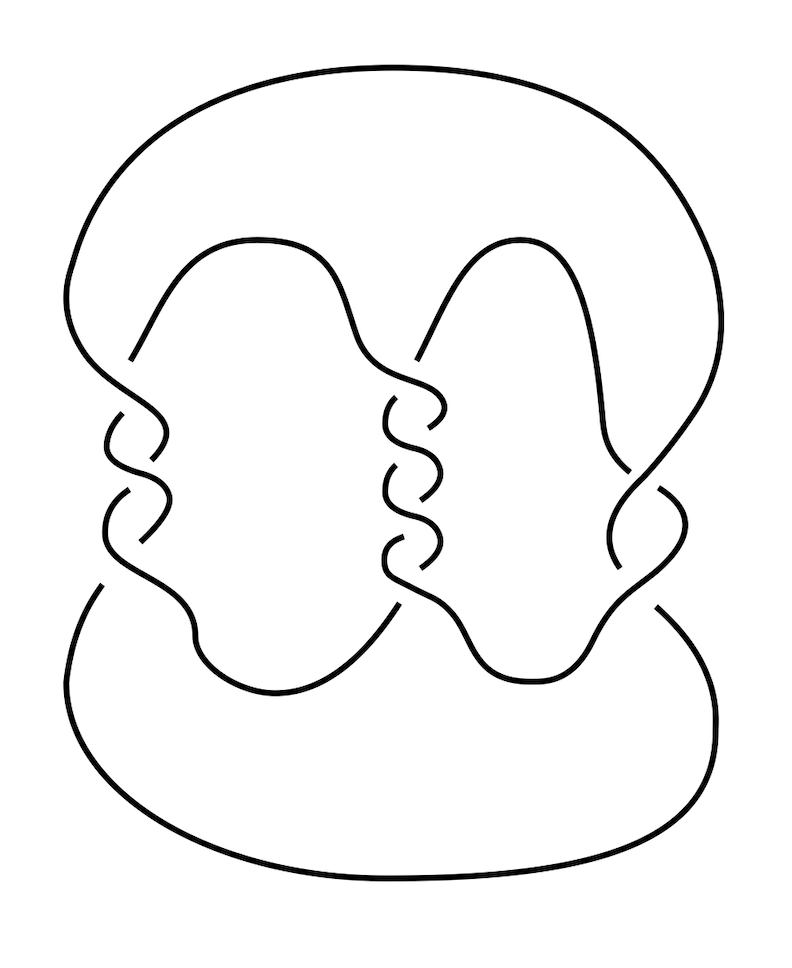
\includegraphics[height=4cm]{augmentation1.png}
\;\;\;\;
& 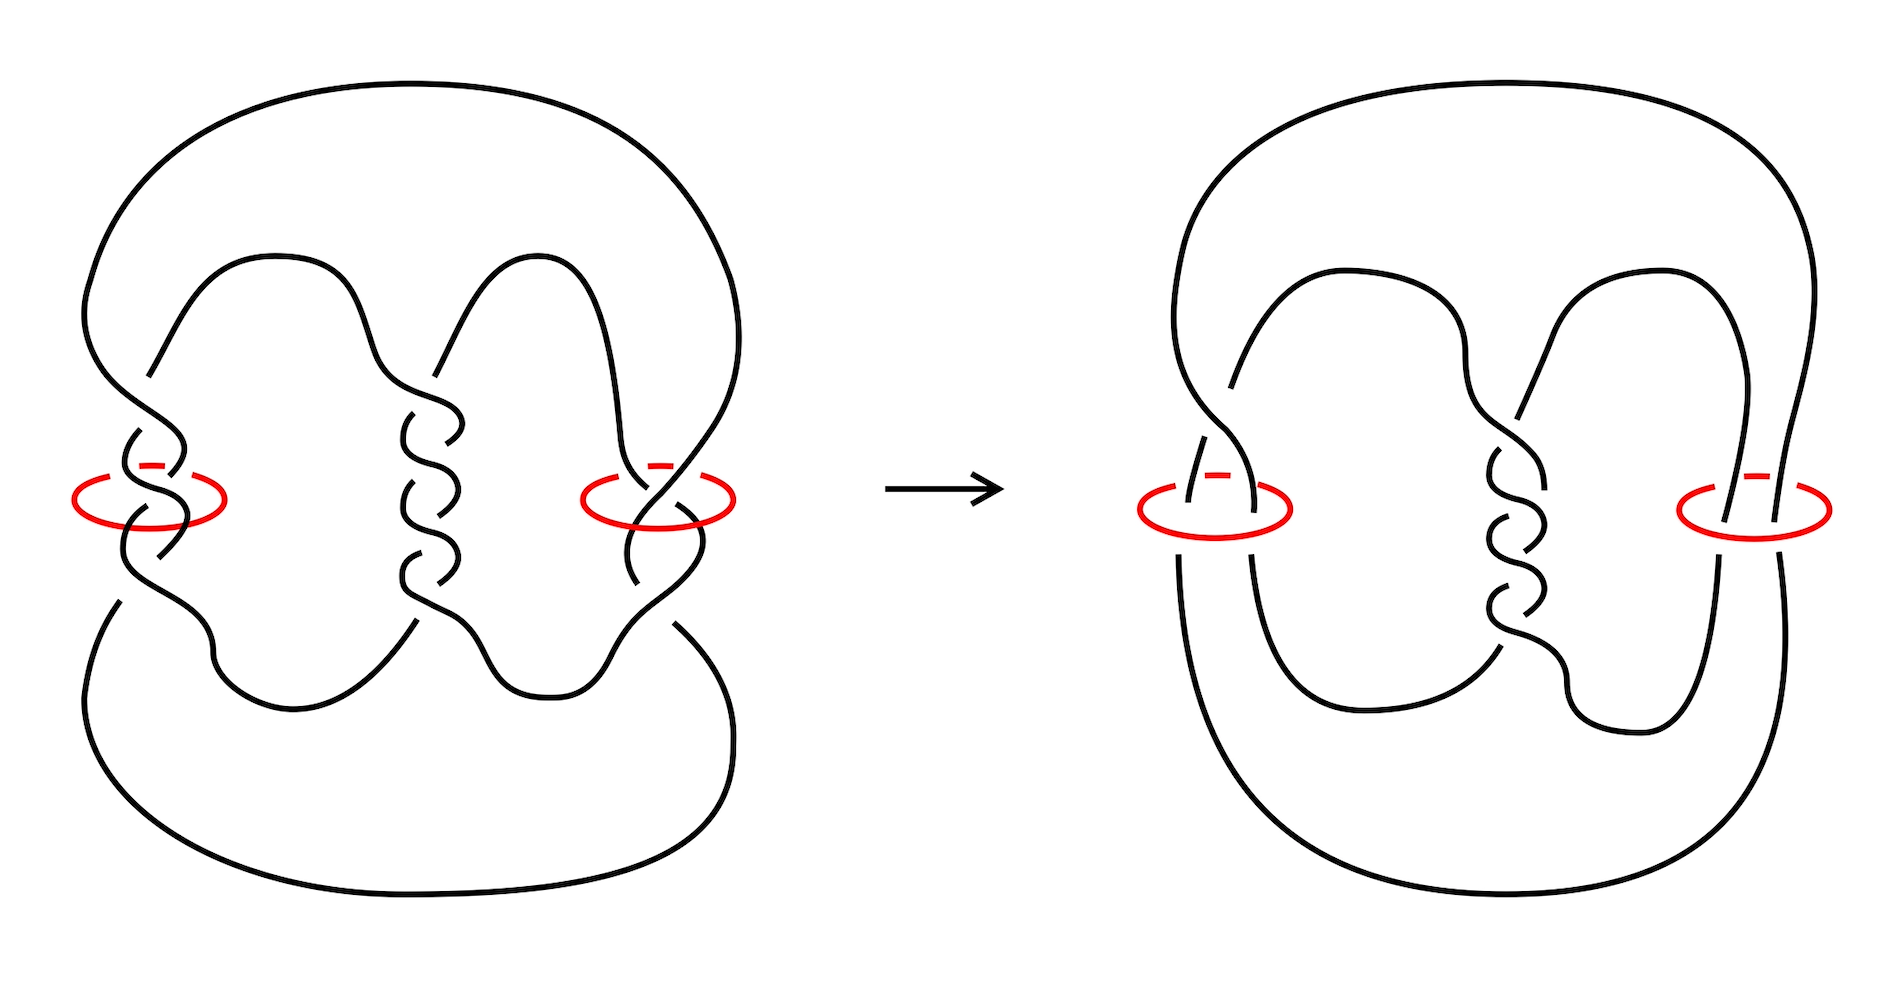
\includegraphics[height=4cm]{augmentation2.png}
\\
(a)
& (b)
\end{tabular}
\caption{(a) pretzel knot before augmentation
(b) pretzel knot after augmentation;
second diagram shows
removal of full twists in the augmented twist regions.}
\label{fig:augmentationS3}
\end{figure}
 
 
 %%%%%%%%%%%%%%%%%%%%%%%%%%%%%%%%%%%%%%%%%%%%%%%%%%%%%%%% 
\section{Augmented Links}
\label{s:auglinks}

TODO Notation section: $I = (-1,1)$.

Champanerkar, Kofman and Purcell have studied alternating links in the thickened
torus \cite{CKP2}. They define a link in the thickened torus as a quotient of a
biperiodic alternating link as follows:
 
\begin{define}
\label{def:biperiodiclink}
A \emph{biperiodic alternating link} $\cL$ is an infinite link
in $\R^2 \times I$ with a link diagram $\cD \subset \R^2$
such that $\cL$ and $\cD$ are
invariant under the action of a two dimensional lattice $\Lambda$
on $\R^2$ by translations.


The quotient $L=\mathcal{L}/\Lambda$ is an alternating link in
the thickened torus $\torus \times I$,
whose projection onto $\torus \times \{0\} = \R^2 \times \{0\} /\Lambda$
is an alternating link diagram $\cD/\Lambda$.
\end{define}


We refer to $\torus \times \{0\}$ as the \emph{projection plane}.


\begin{remark}
Since $\torus \times I \cong \Sp^3 - H$, where $H$ is a Hopf link.
The complement $\torus \times I- L = \Sp^3 - (L \cup H)$.
\end{remark}

Champanerkar, Kofman and Purcell \cite{CKP2} extended
the definition of prime links in $\Sp^3$
for links in $\torus \times I$ called weakly prime. 

\begin{define} \label{def:weaklyprime}
A diagram $D \subset \torus$
of a link $L$ in the thickened torus $\torus \times I$
is \emph{weakly prime}
if whenever a disk is embedded in $\torus$
meets the diagram transversely in exactly two edges,
then the disk contains a simple edge of the diagram and no crossings.
\end{define}


\begin{define}
Recall that a \emph{twist region}
in a link diagram is a maximal sequence of vertices
such that consecutive vertices are two vertices of a bigon face,
and consecutive bigons meet only at a vertex (not an edge).
We say that the \emph{direction} of a twist region
is the pair of faces (possibly the same face)
that are across from the bigons at the end;
if a twist region consists of only one vertex,
a direction is a pair of opposite faces (again, possibly the same face)
meeting at the crossing.
We say that a twist region consisting of only one vertex
is \emph{trivial}.
%%\footnote{There is an ambiguity of ``maximality'' in this definition:
%%for example, if a vertex of a link diagram meets exactly one bigon,
%%it can be considered as part of a twist region of length 2
%%(given by that bigon),
%%or it can be considered as part of a twist region of length 1,
%%as there are no bigons in the other ``direction''.
%%It should be clear which ``direction'' a twist region is going
%%when we deal with augmentations later.
%%}


For links in the thickened torus,
a \emph{twist region} in a link diagram of $L=\mathcal{L}/\Lambda$ in $\torus
\times I$, is the quotient of a twist region in the biperiodic link
$\mathcal{L}$. 


A biperiodic link
$\mathcal{L}$ is called \emph{twist-reduced} if for any simple closed curve on
the plane that intersects the diagram of $\mathcal{L}$
transversely in four points, with two
points adjacent to one crossing and the other two points adjacent to another
crossing, the simple closed curve bounds a subdiagram consisting of a (possibly
empty) collection of bigons strung end to end between these crossings. We say
the diagram of $L$ is \emph{twist-reduced}
if it is the quotient of a twist-reduced biperiodic
link diagram.
\end{define}


We note that when a link diagram is cellular
(Definition \ref{d:cellular}),
a twist region in the torus cannot be a cycle;
otherwise, the face adjacent to the twist region would be an annulus.


Now we can define augmentation for a link in $\torus \times I$ the same way we
define augmentation for links in $\Sp^3$:
%For a link in $\torus \times I$, the
%crossing circles are added to the diagram projected onto $\torus \times \{0\}$.
%Let $D(L)$ be a twist-reduced diagram of a link $L$ in $\torus \times I$, we define
%\emph{augmenting} as a process in which an unknotted circle component is added
%to one or more twist regions of $D(L)$. See Figure \ref{fig:Augmentations}

\begin{definition}
Let $D(K)$ be a twist-reduced diagram of a link $K$ in $\torus \times I$.
We define
\emph{augmenting} as a process in which an unknotted circle component,
called a \emph{crossing circle},
is added to one or more twist regions of $D(K)$
(see Figure \ref{fig:Augmentations});
we call the resulting link $L$ an \emph{augmented link obtained from $K$}.
We say $L$ is \emph{fully} augmented if $L$ is obtained by augmenting
$K$ at \emph{every} crossing/twist site.
\label{d:augmentation}
\end{definition}


As pointed out in the introduction,
after augmenting a twist region,
a standard Dehn twist argument allows us to remove
a full twist (that is, two bigons).

\begin{definition}
We say an augmentation has a \emph{half twist}
if at least one of the augmented twist regions
has an odd number of vertices (i.e. even number of bigons).
\label{d:half-twist}
\end{definition}



\begin{definition}
A graph $G = (V,E)$ on the torus is \emph{cellular}
if its complement is a collection of open disks.
\label{d:cellular}
\end{definition}

%We say that a link diagram in the thickened torus is
%\emph{cellular}.

%%\begin{remark}
%%If $L$ is augmented at \emph{every} crossing/twist site we say $L$ is \emph{fully} augmented.
%%\end{remark}


\begin{figure}
\centering
\begin{tabular}{cccc}
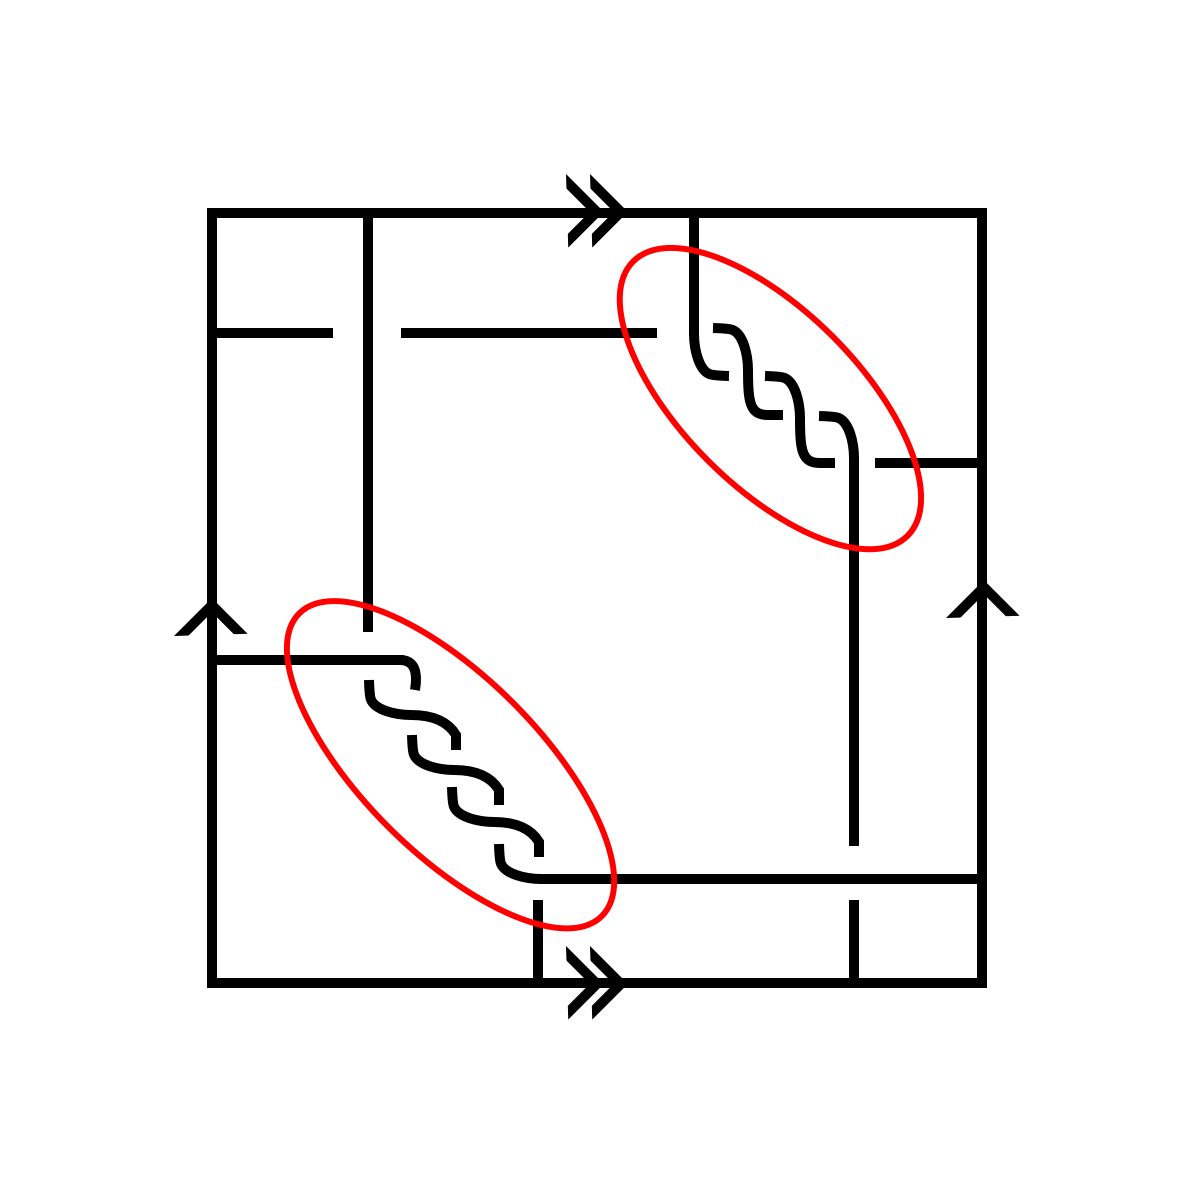
\includegraphics[width=3cm]{fig1.png}&
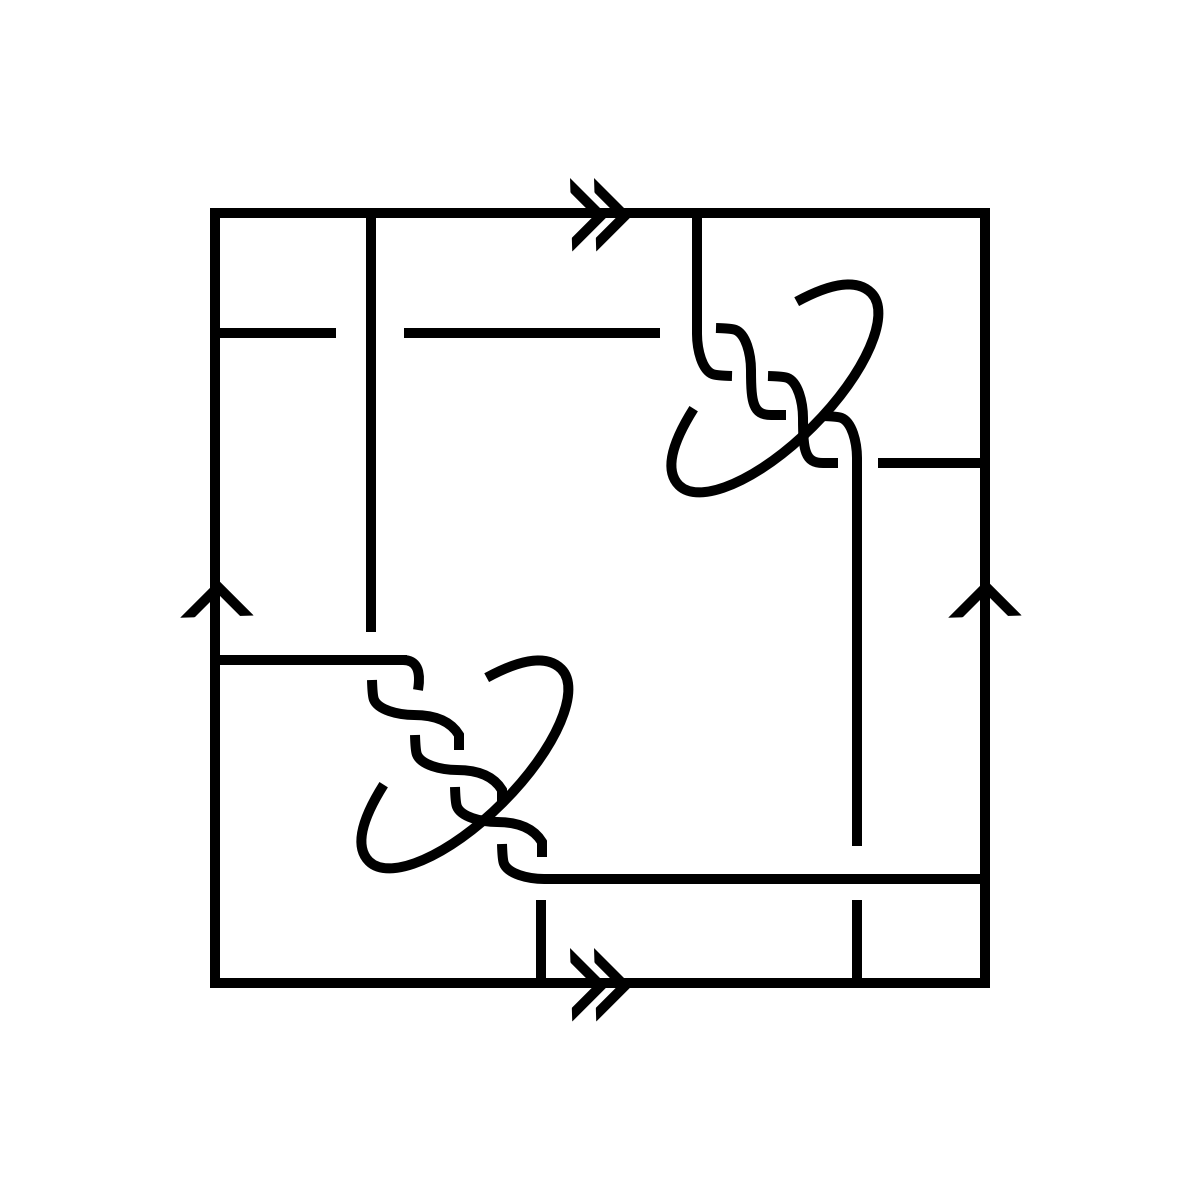
\includegraphics[width=3cm]{twist-augment.png}&
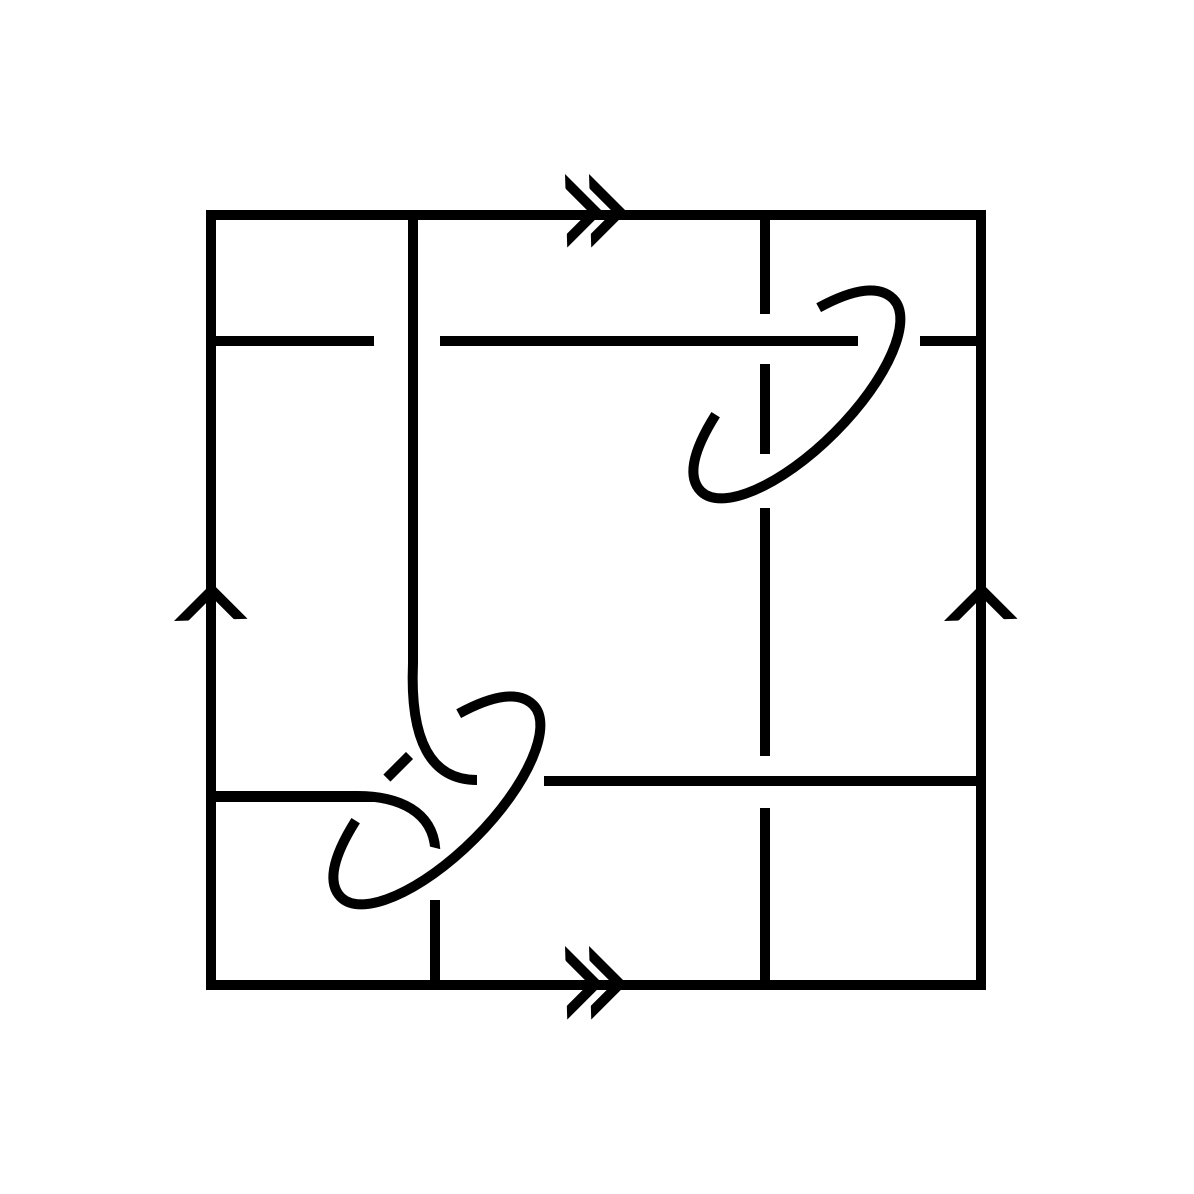
\includegraphics[width=3cm]{fig-2.png}\\
 % 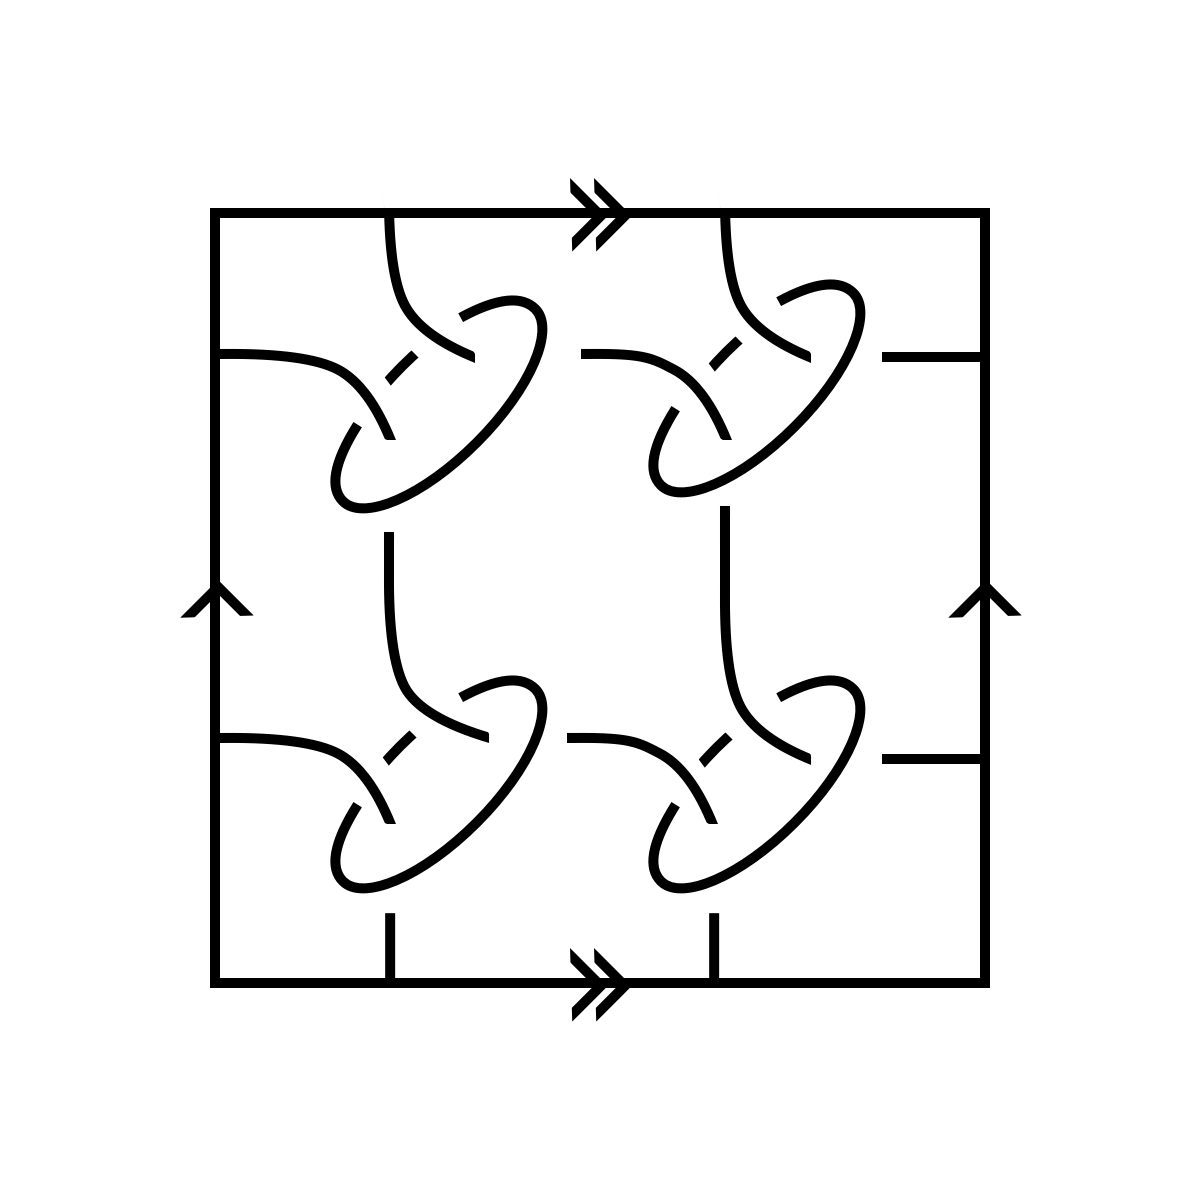
\includegraphics [width=3cm]{fal}\\
A&B&C
\end{tabular}
	 \caption{A: The top right has an odd number of twists while the bottom left has
	 an even number of twists. B: The picture of the link on the right after
	 augmentation twist regions circled in red. C: The link with full twists
	 removed.}
\label{fig:Augmentations}
\end{figure}
%%%%%%%%%%%%%%%%%%%%%%%%%%%%%%%%%%%%%%%%%%%%%%%%%%%% 

\subsection{Torihedral Decomposition of Augmented Alternating Links in Thickened Torus}


We present a method of decomposing an augmented link
(not necessarily fully augmented) in the thickened torus into
objects called ``torihedra'' as defined below.
Decomposing alternating links in the thickened torus into 
torihedra were first described in \cite{CKP2},
then later used for fully augmented links in 
the thickened torus in \cite{kwon2020fully}.
The idea is to combine methods of Menasco
\cite{Menasco} and the use of crossing edges
between (TODO for?) each crossing of our link
and Lackenby's ``cut-slice-flatten" method \cite{lackenby}
on the augmentation
sites.



\begin{define}\cite{CKP2}
\label{def:torihedron}
A \emph{torihedron} $\sT$ is a cone on the torus, 
i.e. $\torus \times [0,1]/(\torus \times \{1\})$, with a cellular graph
$G = G(\sT)$ on $\torus \times \{0\}$.
The \emph{ideal torihedron} $\sT^\circ$ is $\sT$ with the
vertices of $G$ and the vertex $\torus \times \{1\}$ removed. Hence, an ideal
torihedron is homeomorphic to $\torus \times [0,1)$ with a finite set of points
(ideal vertices) removed from $\torus \times \{0\}$.
We refer to the vertex $\torus \times \{1\}$ as the \emph{cone point}
of $\sT$.
\end{define}


For visualization purposes, we typically draw the graph $G(\sT)$ of a
torihedron from the perspective of the cone point $\torus \times \{1\}$.
Note however that later we will be dealing with
``top'' and ``bottom'' torihedra that are glued together
along their torus boundary faces;
to avoid confusion, we will visualize the graphs of both torihedra
from the perspective of the cone point of the ``top'' torihedron.


If the faces of $G(\sT)$ are disks,
then $\sT$ can be decomposed into a union of pyramids,
obtained by coning each face to the cone point of $\sT$.
This also gives a decomposition of the corresponding ideal torihedron
$\sT^\circ$ into ideal pyramids.
We call these the \emph{pyramidal decompositions} of $\sT$ and $\sT^\circ$.


\begin{definition}
Let $G$ be a graph on the torus.
Let $v$ be a vertex and $e,e'$ be distinct edges that meet $v$.
A \emph{left (resp. right) bow-tie modification to $v,e,e'$}
is the process of removing $v,e,e'$ and adding in a ``bow-tie''
as in Figure \ref{TODO} (a) (resp. (b)).
We call the TODO \emph{long} edges, the TODO \emph{short} edges,
and TODO \emph{diagonal} edges,
and we call the new triangular faces the \emph{bow-tie faces}.
TODO in figure caption, left bow-tie modification so-called because
the triangular face appears to the left of the long edges;
also note that left/right conincide with Figure \ref{f:right_left_aug}


\begin{figure}[ht]
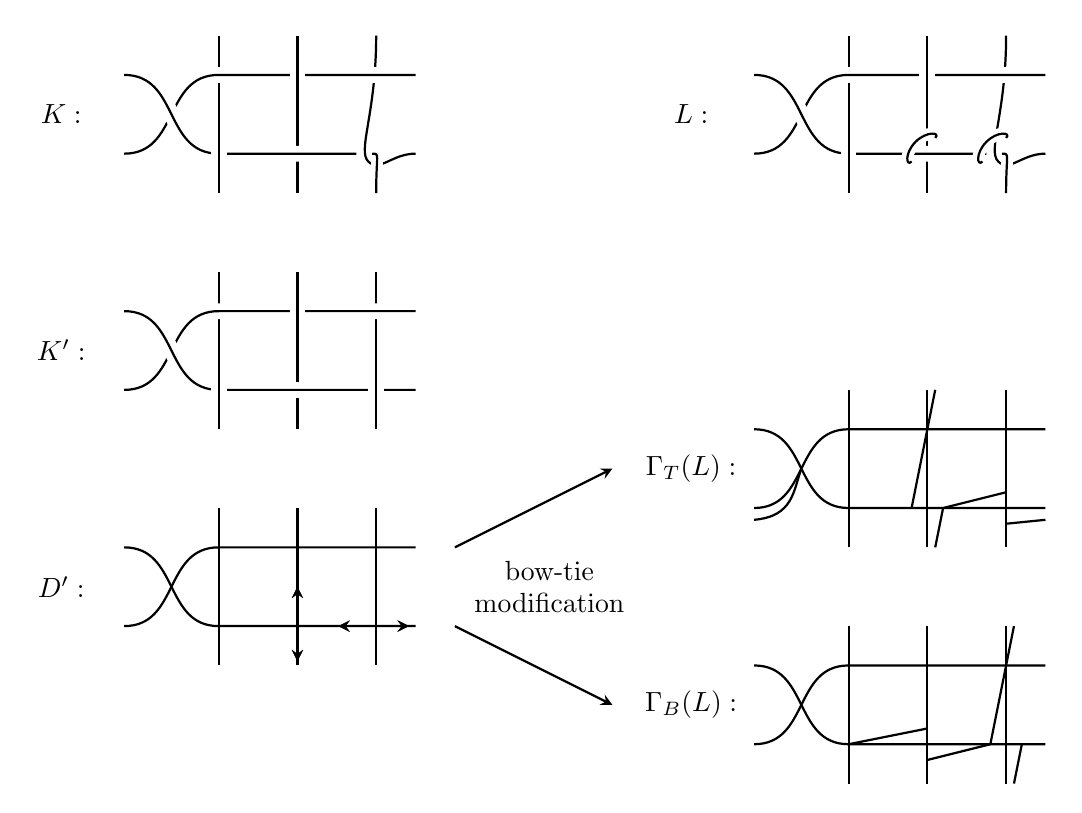
\begin{tikzpicture}
\begin{scope}[shift={(0,0)}]
\node at (-2,0.5) {$K:$};
%% vertical lines
\draw (0,-0.5) -- (0,1.5);
\draw (1,-0.5) -- (1,1.5);
%\draw (2,-0.5) -- (2,1.5);
\draw (2,1.5)
	.. controls +(-90:1cm) and +(135:0.2cm) .. (1.9,-0.1)
	.. controls +(-45:0.2cm) and +(180:0.3cm) .. (2.5,0);
%$% horizontal lines
\draw[overline] (-1.2,0)
	.. controls +(0:0.7cm) and +(180:0.7cm) .. (0,1)
	-- (2.5,1);
\draw[overline] (-1.2,1)
	.. controls +(0:0.7cm) and +(180:0.7cm) .. (0,0)
	-- (1.75,0);
\draw[thin_overline={1.5}] (1.95,0)
	.. controls +(0:0.1cm) and +(90:0.5cm) .. (2,-0.5);
%% vertical lines again
\draw[overline] (0,-0.5) -- (0,0.5);
\draw[overline] (1,0.5) -- (1,1.5);
%\draw[overline] (2,-0.5) -- (2,0.5);
\end{scope}
%%%%%%%%%%%%%%%%%%%%%%%%%%%%%%%%%%%%%%%%%%%%%%
\begin{scope}[shift={(8,0)}]
\node at (-2,0.5) {$L:$};
%% vertical lines
\draw (0,-0.5) -- (0,1.5);
\draw (1,-0.5) -- (1,1.5);
%\draw (2,-0.5) -- (2,1.5);
\draw (2,1.5)
	.. controls +(-90:1cm) and +(135:0.2cm) .. (1.9,-0.1)
	.. controls +(-45:0.2cm) and +(180:0.3cm) .. (2.5,0);
%$% horizontal lines
\draw[overline] (-1.2,0)
	.. controls +(0:0.7cm) and +(180:0.7cm) .. (0,1)
	-- (2.5,1);
\draw[overline] (-1.2,1)
	.. controls +(0:0.7cm) and +(180:0.7cm) .. (0,0)
	-- (1.75,0);
\draw[thin_overline={1.5}] (1.95,0)
	.. controls +(0:0.1cm) and +(90:0.5cm) .. (2,-0.5);
%% vertical lines again
\draw[overline] (0,-0.5) -- (0,0.5);
\draw[overline] (1,0.5) -- (1,1.5);
%\draw[overline] (2,-0.5) -- (2,0.5);
%% augmentations/crossing circles
\draw[thin_overline={1.5}] (0.8,-0.1)
	.. controls +(-135:0.1cm) and +(-135:0.2cm) .. (0.85,0.15)
	.. controls +(45:0.2cm) and +(45:0.1cm) .. (1.1,0.2);
\draw[thin_overline={1.5}] (1.7,-0.1)
	.. controls +(-135:0.1cm) and +(-135:0.2cm) .. (1.75,0.15)
	.. controls +(45:0.2cm) and +(45:0.1cm) .. (2,0.2);
\end{scope}
%%%%%%%%%%%%%%%%%%%%%%%%%%%%%%%%%%%%%%%%%%%%%%
\begin{scope}[shift={(0,-3)}]
\node at (-2,0.5) {$K':$};
%% vertical lines
\draw (0,-0.5) -- (0,1.5);
\draw (1,-0.5) -- (1,1.5);
\draw (2,-0.5) -- (2,1.5);
%$% horizontal lines
\draw[overline] (-1.2,0)
	.. controls +(0:0.7cm) and +(180:0.7cm) .. (0,1)
	-- (2.5,1);
\draw[overline] (-1.2,1)
	.. controls +(0:0.7cm) and +(180:0.7cm) .. (0,0)
	-- (2.5,0);
%% vertical lines again
\draw[overline] (0,-0.5) -- (0,0.5);
\draw[overline] (1,0.5) -- (1,1.5);
\draw[overline] (2,-0.5) -- (2,0.5);
\end{scope}
%%%%%%%%%%%%%%%%%%%%%%%%%%%%%%%%%%%%%%%%%%%%%%
%% D' diagram
\begin{scope}[shift={(0,-6)}]
\node at (-2,0.5) {$D':$};
%% vertical lines
\draw (0,-0.5) -- (0,1.5);
\draw[midarrow_rev={0.1},midarrow={0.5}]  (1,-0.5) -- (1,1.5);
\draw (2,-0.5) -- (2,1.5);
%% horizontal lines
\draw (-1.2,0)
	.. controls +(0:0.7cm) and +(180:0.7cm) .. (0,1)
	-- (2.5,1);
\draw[midarrow_rev={0.8},midarrow={0.98}] (-1.2,1)
	.. controls +(0:0.7cm) and +(180:0.7cm) .. (0,0)
	-- (2.5,0);
%% arrow label
\draw[->] (3,1) -- (5,2);
\draw[->] (3,0) -- (5,-1);
\node at (4.2,0.7) {bow-tie};
\node at (4.2,0.3) {modification};
\end{scope}
%%%%%%%%%%%%%%%%%%%%%%%%%%%%%%%%%%%%%%%%%%%%%%
%% top torihedron graph
\begin{scope}[shift={(8,-4.5)}]
\node at (-2,0.5) {$\Gamma_T(L):$};
%% vertical lines
\draw (0,-0.5) -- (0,1.5);
\draw (1,-0.5) -- (1,1.5);
\draw (2,-0.5) -- (2,1.5);
%% horizontal lines
\draw (-1.2,0)
	.. controls +(0:0.7cm) and +(180:0.7cm) .. (0,1)
	-- (2.5,1);
\draw (-1.2,1)
	.. controls +(0:0.7cm) and +(180:0.7cm) .. (0,0)
	-- (2.5,0);
%% bow-tie
\draw (0.8,0) -- (1,1);
\draw (1.2,0) -- (1.1,-0.5);
\draw (1.1,1.5) -- (1,1);
%% second bow-tie
\draw (1.2,0) -- (2,0.2);
\draw (2,-0.2) -- (2.5,-0.15);
\draw (-1.2,-0.15)
	.. controls +(5:0.5cm) and +(-110:0.3cm) .. (-0.6,0.5);
\end{scope}
%%%%%%%%%%%%%%%%%%%%%%%%%%%%%%%%%%%%%%%%%%%%%%
%% bottom torihedron graph
\begin{scope}[shift={(8,-7.5)}]
\node at (-2,0.5) {$\Gamma_B(L):$};
%% vertical lines
\draw (0,-0.5) -- (0,1.5);
\draw (1,-0.5) -- (1,1.5);
\draw (2,-0.5) -- (2,1.5);
%% horizontal lines
\draw (-1.2,0)
	.. controls +(0:0.7cm) and +(180:0.7cm) .. (0,1)
	-- (2.5,1);
\draw (-1.2,1)
	.. controls +(0:0.7cm) and +(180:0.7cm) .. (0,0)
	-- (2.5,0);
%% bow-tie
\draw (0,0) -- (1,0.2);
\draw (1,-0.2) -- (1.8,0);
%% second bow-tie
\draw (1.8,0) -- (2,1);
\draw (2.2,0) -- (2.1,-0.5);
\draw (2.1,1.5) -- (2,1);
\end{scope}
\end{tikzpicture}


\caption{Bow-tie modifications}
\label{f:bow-tie-modification}
\end{figure}


\label{d:diagram-bowtie}
\end{definition}


\begin{define}
We say a twist region is \emph{right-augmented} if, when both strands are
(locally) oriented so that they cross the augmentation disk in the same
direction, the crossing is a positive right-handed half-twist.
We say a twist is \emph{left-augmented} if it is not right-augmented.
See Figure \ref{f:right_left_aug}.
\end{define}


We can recover $L$ from the link diagram of $K$
together with labels at twist regions indicating left- or right-augmentation.

\begin{definition}
\label{d:tori-decomp-graph}
Let $L$ be a link obtained from augmenting an alternating link $K$
with a cellular link diagram $D = D(K)$.
We define the \emph{top/bottom bow-tie graph of $L$} as follows.


%Let $D = D(K)$ be the link diagram of $K$,
Let $D'$ be the graph obtained from $D$
by collapsing each augmented twist region of $K$ to a vertex.
Clearly, $D'$ is the link diagram of a link $K'$
obtained from $K$ by removing half-twists from each augmented twist region
until one crossing remains.
Let $v_t$ denote a vertex of $D'$ corresponding to
an augmented twist region of $K$,
and let $v_c$ denote a vertex of $D'$ corresponding to
a crossing of $K$ not in an augmented twist region.


Orient the edges of $D'$ to point from an undercrossing
to an overcrossing.
Label the two outgoing edges at vertex $v$
(which corresponds to a crossing or a twist region)
by $e_v^{(1)}, e_v^{(2)}$ (in arbitrary order).
For each left- (resp. right-) augmented twist region $t$,
we perform a left (resp. right) bow-tie modification to
$v_t, e_{v_t}^{(1)}, e_{v_t}^{(2)}$.


We call the resulting graph the \emph{top bow-tie graph of $L$},
denoted by $\Gamma_T(L)$.
If we had oriented the edges of $D'$ the other way,
and subsequently performed the same operations,
we obtain another graph,
which we call the \emph{bottom bow-tie graph of $L$},
denoted by $\Gamma_B(L)$.
%\hfill $\triangle$
\end{definition}

\begin{figure}[ht]
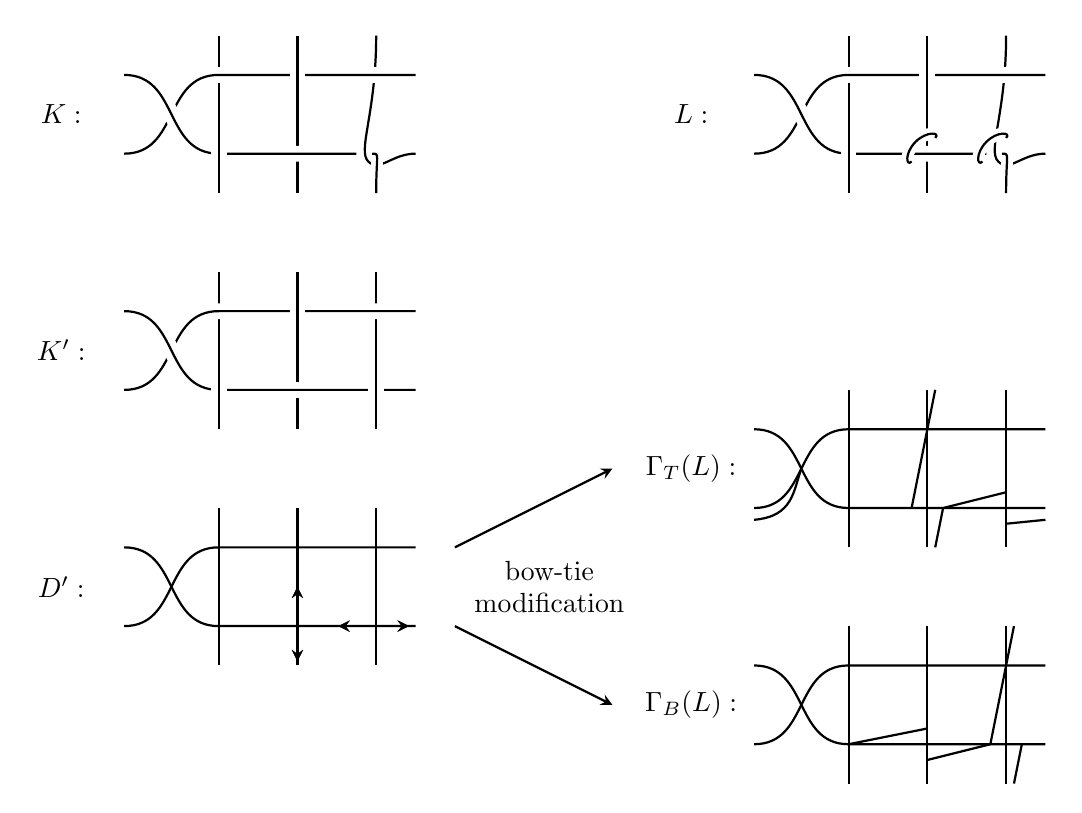
\begin{tikzpicture}
\begin{scope}[shift={(0,0)}]
\node at (-2,0.5) {$K:$};
%% vertical lines
\draw (0,-0.5) -- (0,1.5);
\draw (1,-0.5) -- (1,1.5);
%\draw (2,-0.5) -- (2,1.5);
\draw (2,1.5)
	.. controls +(-90:1cm) and +(135:0.2cm) .. (1.9,-0.1)
	.. controls +(-45:0.2cm) and +(180:0.3cm) .. (2.5,0);
%$% horizontal lines
\draw[overline] (-1.2,0)
	.. controls +(0:0.7cm) and +(180:0.7cm) .. (0,1)
	-- (2.5,1);
\draw[overline] (-1.2,1)
	.. controls +(0:0.7cm) and +(180:0.7cm) .. (0,0)
	-- (1.75,0);
\draw[thin_overline={1.5}] (1.95,0)
	.. controls +(0:0.1cm) and +(90:0.5cm) .. (2,-0.5);
%% vertical lines again
\draw[overline] (0,-0.5) -- (0,0.5);
\draw[overline] (1,0.5) -- (1,1.5);
%\draw[overline] (2,-0.5) -- (2,0.5);
\end{scope}
%%%%%%%%%%%%%%%%%%%%%%%%%%%%%%%%%%%%%%%%%%%%%%
\begin{scope}[shift={(8,0)}]
\node at (-2,0.5) {$L:$};
%% vertical lines
\draw (0,-0.5) -- (0,1.5);
\draw (1,-0.5) -- (1,1.5);
%\draw (2,-0.5) -- (2,1.5);
\draw (2,1.5)
	.. controls +(-90:1cm) and +(135:0.2cm) .. (1.9,-0.1)
	.. controls +(-45:0.2cm) and +(180:0.3cm) .. (2.5,0);
%$% horizontal lines
\draw[overline] (-1.2,0)
	.. controls +(0:0.7cm) and +(180:0.7cm) .. (0,1)
	-- (2.5,1);
\draw[overline] (-1.2,1)
	.. controls +(0:0.7cm) and +(180:0.7cm) .. (0,0)
	-- (1.75,0);
\draw[thin_overline={1.5}] (1.95,0)
	.. controls +(0:0.1cm) and +(90:0.5cm) .. (2,-0.5);
%% vertical lines again
\draw[overline] (0,-0.5) -- (0,0.5);
\draw[overline] (1,0.5) -- (1,1.5);
%\draw[overline] (2,-0.5) -- (2,0.5);
%% augmentations/crossing circles
\draw[thin_overline={1.5}] (0.8,-0.1)
	.. controls +(-135:0.1cm) and +(-135:0.2cm) .. (0.85,0.15)
	.. controls +(45:0.2cm) and +(45:0.1cm) .. (1.1,0.2);
\draw[thin_overline={1.5}] (1.7,-0.1)
	.. controls +(-135:0.1cm) and +(-135:0.2cm) .. (1.75,0.15)
	.. controls +(45:0.2cm) and +(45:0.1cm) .. (2,0.2);
\end{scope}
%%%%%%%%%%%%%%%%%%%%%%%%%%%%%%%%%%%%%%%%%%%%%%
\begin{scope}[shift={(0,-3)}]
\node at (-2,0.5) {$K':$};
%% vertical lines
\draw (0,-0.5) -- (0,1.5);
\draw (1,-0.5) -- (1,1.5);
\draw (2,-0.5) -- (2,1.5);
%$% horizontal lines
\draw[overline] (-1.2,0)
	.. controls +(0:0.7cm) and +(180:0.7cm) .. (0,1)
	-- (2.5,1);
\draw[overline] (-1.2,1)
	.. controls +(0:0.7cm) and +(180:0.7cm) .. (0,0)
	-- (2.5,0);
%% vertical lines again
\draw[overline] (0,-0.5) -- (0,0.5);
\draw[overline] (1,0.5) -- (1,1.5);
\draw[overline] (2,-0.5) -- (2,0.5);
\end{scope}
%%%%%%%%%%%%%%%%%%%%%%%%%%%%%%%%%%%%%%%%%%%%%%
%% D' diagram
\begin{scope}[shift={(0,-6)}]
\node at (-2,0.5) {$D':$};
%% vertical lines
\draw (0,-0.5) -- (0,1.5);
\draw[midarrow_rev={0.1},midarrow={0.5}]  (1,-0.5) -- (1,1.5);
\draw (2,-0.5) -- (2,1.5);
%% horizontal lines
\draw (-1.2,0)
	.. controls +(0:0.7cm) and +(180:0.7cm) .. (0,1)
	-- (2.5,1);
\draw[midarrow_rev={0.8},midarrow={0.98}] (-1.2,1)
	.. controls +(0:0.7cm) and +(180:0.7cm) .. (0,0)
	-- (2.5,0);
%% arrow label
\draw[->] (3,1) -- (5,2);
\draw[->] (3,0) -- (5,-1);
\node at (4.2,0.7) {bow-tie};
\node at (4.2,0.3) {modification};
\end{scope}
%%%%%%%%%%%%%%%%%%%%%%%%%%%%%%%%%%%%%%%%%%%%%%
%% top torihedron graph
\begin{scope}[shift={(8,-4.5)}]
\node at (-2,0.5) {$\Gamma_T(L):$};
%% vertical lines
\draw (0,-0.5) -- (0,1.5);
\draw (1,-0.5) -- (1,1.5);
\draw (2,-0.5) -- (2,1.5);
%% horizontal lines
\draw (-1.2,0)
	.. controls +(0:0.7cm) and +(180:0.7cm) .. (0,1)
	-- (2.5,1);
\draw (-1.2,1)
	.. controls +(0:0.7cm) and +(180:0.7cm) .. (0,0)
	-- (2.5,0);
%% bow-tie
\draw (0.8,0) -- (1,1);
\draw (1.2,0) -- (1.1,-0.5);
\draw (1.1,1.5) -- (1,1);
%% second bow-tie
\draw (1.2,0) -- (2,0.2);
\draw (2,-0.2) -- (2.5,-0.15);
\draw (-1.2,-0.15)
	.. controls +(5:0.5cm) and +(-110:0.3cm) .. (-0.6,0.5);
\end{scope}
%%%%%%%%%%%%%%%%%%%%%%%%%%%%%%%%%%%%%%%%%%%%%%
%% bottom torihedron graph
\begin{scope}[shift={(8,-7.5)}]
\node at (-2,0.5) {$\Gamma_B(L):$};
%% vertical lines
\draw (0,-0.5) -- (0,1.5);
\draw (1,-0.5) -- (1,1.5);
\draw (2,-0.5) -- (2,1.5);
%% horizontal lines
\draw (-1.2,0)
	.. controls +(0:0.7cm) and +(180:0.7cm) .. (0,1)
	-- (2.5,1);
\draw (-1.2,1)
	.. controls +(0:0.7cm) and +(180:0.7cm) .. (0,0)
	-- (2.5,0);
%% bow-tie
\draw (0,0) -- (1,0.2);
\draw (1,-0.2) -- (1.8,0);
%% second bow-tie
\draw (1.8,0) -- (2,1);
\draw (2.2,0) -- (2.1,-0.5);
\draw (2.1,1.5) -- (2,1);
\end{scope}
\end{tikzpicture}


\caption{Constructing the top and bottom bow-tie graphs,
using bow-tie modifications}
\label{f:tori-decomp-graph}
\end{figure}

Note that the non-bow-tie faces of $\Gamma_T(L)$ and $\Gamma_B(L)$
are naturally identified with the faces of $D'$
(as the bow-tie modification procedure does not remove faces).


\begin{prop}\label{p:tori_decomp}
Let $K$ be an alternating link in the thickened torus
with a cellular link diagram,
and let $L$ be an augmented link obtained from $K$.
%Let $G(L)$ be a diagram of the link on $\torus \times \{0\}$.
There is a decomposition of the complement,
$(\torus \times I) - L$, into two ideal torihedra;
the graphs of the torihedra are $\Gamma_T(L)$ and $\Gamma_B(L)$.
\end{prop}


\begin{proof}
%As mentioned before, we will be combining
%Menasco's method using crossing edges at each crossing
%and Lackenby's ``cut-slice-flatten'' method
%on augmentation sites.

%We give a description of the topological operations
%that give the torihedral decomposition;
%this will justify the 
%more concise description purely in terms of link diagrams
%which we present in Remark \ref{r:tori-decomp-graph}.


We will begin by assuming that $L$ has no half twists.
Let $L = K \cup C$, with $C$ being the collection of crossing circles.
%Arrange the link diagram of $L$ in the following way:
Arrange $L$ in the following way:
place the circle components in $C$ perpendicular to
the projection plane $\torus \times \{0\}$,
and leave the remaining part of the link $K \subseteq L$
lying in the projection plane (except at crossings of $K$).
Thus, the projection of $L$ onto the projection plane
will be a diagram $D(K)$ of $K$
together with line segments corresponding to crossing circles.
%(We demand that $D(K)$ be alternating and twist-reduced.)
As discussed before, we may remove full twists (i.e. pairs of bigons)
from the twist regions of $K$ that are augmented in $L$,
and since $L$ is assumed to have no half twists,
the two edges of $D(K)$ that go through a crossing circle
do not meet (see Figure \ref{fig:Augmentations} C).
From now on, we will take $K$ to be this modified link
(with full twists removed).


We now place a \emph{crossing edge} at each crossing of $K$,
connecting the top and bottom strands at the crossing
(see \figref{f:crossing-edges}).
%(see Figure \ref{fig:crossingArc} (a)).
%so that for each crossing edge,
%one end of the edge lies on a bottom strand while the other
%end lies on a top strand as in Figure \ref{fig:crossingArc} (a).

\begin{figure} 
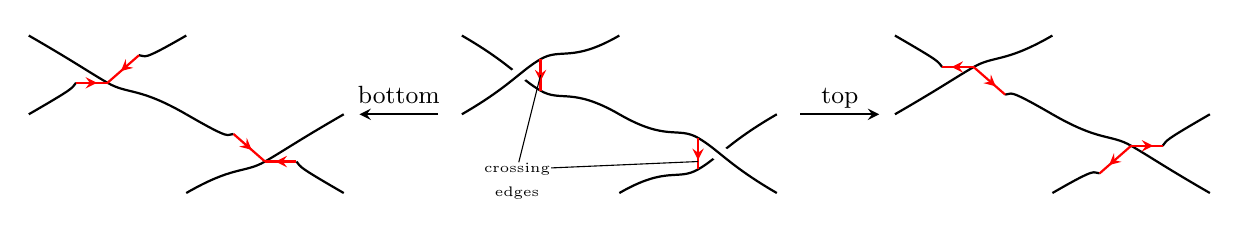
\begin{tikzpicture}
\begin{scope}[shift={(0,0)}]
\draw (2,-1)
	.. controls +(30:0.7cm) and +(-150:0.3cm) .. (3,-0.7)
	.. controls +(30:0.3cm) and +(-150:0.7cm) .. (4,0);
\draw[overline] (2,0)
	.. controls +(-30:0.7cm) and +(150:0.3cm) .. (3,-0.3)
	.. controls +(-30:0.3cm) and +(150:0.7cm) .. (4,-1);
\draw (0,1)
	.. controls +(-30:0.7cm) and +(150:0.3cm) .. (1,0.3)
	.. controls +(-30:0.3cm) and +(150:0.7cm) .. (2,0);
\draw[overline] (0,0)
	.. controls +(30:0.7cm) and +(-150:0.3cm) .. (1,0.7)
	.. controls +(30:0.3cm) and +(-150:0.7cm) .. (2,1);
%% crossing edges
\draw[color=red,midarrow={0.7}] (1,0.7) -- (1,0.3);
\draw[color=red,midarrow={0.7}] (3,-0.3) -- (3,-0.7);
%% label
\node[inner sep=0] (x) at (0.7,-0.7) {\tiny crossing};
\node[inner sep=0] (y) at (0.7,-1.0) {\tiny edges};
\draw[line width=0.4pt] (x) -- (1,0.5);
\draw[line width=0.4pt] (x) -- (3,-0.6);
%%%% edge to crossing circle/disc
%%\draw (4,0)
%%	.. controls +(30:0.5cm) and +(-150:0.7cm) .. (4.4,1.2);
%%\draw (2,1)
%%	.. controls +(30:0.5cm) and +(-150:0.7cm) .. (4,1.4);
%%%% crossing circle/disc
%%\filldraw[med-gray] (3.6,1.6) to[out=90,in=90] (4.8,1.0)
%%	-- cycle;
%%\draw (3.6,1.6) to[out=90,in=90] (4.8,1.0);
%%\draw[color=red] (3.6,1.6) -- (4.8,1.0);
%% arrows to left/right diagrams
\draw[->] (-0.3,0) -- (-1.3,0);
\node at (-0.8,0.25) {\small bottom};
\draw[->] (4.3,0) -- (5.3,0);
\node at (4.8,0.2) {\small top};
\end{scope}
%%%%%%%%%%%%%%%%%%%%%%%%%%%%%%%%%%%%%%%%%%%%%%%%%%%%%%%
\begin{scope}[shift={(5.5,0)}]
\node[emptynode] (a) at (2.6,-0.75) {};
\node[emptynode] (b) at (3.4,-0.4) {};
\node[emptynode] (c) at (1.4,0.25) {};
\node[emptynode] (d) at (0.6,0.6) {};
\draw (2,-1)
	.. controls +(30:0.7cm) and +(180:0.1cm) .. (a);
\draw (b)
	.. controls +(50:0.1cm) and +(-150:0.7cm) .. (4,0);
\draw (2,0)
	.. controls +(-30:0.7cm) and +(150:0.3cm) .. (3,-0.4)
	.. controls +(-30:0.3cm) and +(150:0.7cm) .. (4,-1);
\draw (0,1)
	.. controls +(-30:0.7cm) and +(130:0.1cm) .. (d);
\draw (c)
	.. controls +(0:0.1cm) and +(150:0.7cm) .. (2,0);
\draw (0,0)
	.. controls +(30:0.7cm) and +(-150:0.3cm) .. (1,0.6)
	.. controls +(30:0.3cm) and +(-150:0.7cm) .. (2,1);
%% crossing edges
\draw[color=red,midarrow={0.7}] (3,-0.4) -- (a);
\draw[color=red,midarrow={0.7}] (3,-0.4) -- (b);
\draw[color=red,midarrow={0.7}] (1,0.6) -- (c);
\draw[color=red,midarrow={0.7}] (1,0.6) -- (d);
%%%% edge to crossing circle/disc
%%\draw (4,0)
%%	.. controls +(30:0.5cm) and +(-150:0.7cm) .. (4.4,1.2);
%%\draw (2,1)
%%	.. controls +(30:0.5cm) and +(-150:0.7cm) .. (4,1.4);
%%%% crossing circle/disc
%%\filldraw[med-gray] (3.6,1.6) to[out=90,in=90] (4.8,1.0)
%%	-- (4.2,1.0) -- (3.6,1.25) -- cycle;
%%\draw (3.6,1.6) to[out=90,in=90] (4.8,1.0);
%%\draw[color=red] (3.6,1.6) -- (3.6,1.25) -- (4.2,1.0) -- (4.8,1.0);
\end{scope}
%%%%%%%%%%%%%%%%%%%%%%%%%%%%%%%%%%%%%%%%%%%%%%%%%%%%%%%
\begin{scope}[shift={(-1.5,0)},rotate=180]
\node[emptynode] (a) at (2.6,-0.75) {};
\node[emptynode] (b) at (3.4,-0.4) {};
\node[emptynode] (c) at (1.4,0.25) {};
\node[emptynode] (d) at (0.6,0.6) {};
\draw (2,-1)
	.. controls +(30:0.7cm) and +(180:0.1cm) .. (a);
\draw (b)
	.. controls +(50:0.1cm) and +(-150:0.7cm) .. (4,0);
\draw (2,0)
	.. controls +(-30:0.7cm) and +(150:0.3cm) .. (3,-0.4)
	.. controls +(-30:0.3cm) and +(150:0.7cm) .. (4,-1);
\draw (0,1)
	.. controls +(-30:0.7cm) and +(130:0.1cm) .. (d);
\draw (c)
	.. controls +(0:0.1cm) and +(150:0.7cm) .. (2,0);
\draw (0,0)
	.. controls +(30:0.7cm) and +(-150:0.3cm) .. (1,0.6)
	.. controls +(30:0.3cm) and +(-150:0.7cm) .. (2,1);
%% crossing edges
\draw[color=red,midarrow_rev={0.7}] (3,-0.4) -- (a);
\draw[color=red,midarrow_rev={0.7}] (3,-0.4) -- (b);
\draw[color=red,midarrow_rev={0.7}] (1,0.6) -- (c);
\draw[color=red,midarrow_rev={0.7}] (1,0.6) -- (d);
%%%% edge to crossing circle/disc
%%\draw (4,0)
%%	.. controls +(30:0.5cm) and +(-150:0.7cm) .. (4.4,1.2);
%%\draw (2,1)
%%	.. controls +(30:0.5cm) and +(-150:0.7cm) .. (4,1.4);
%%%% crossing circle/disc
%%\filldraw[med-gray] (3.6,1.6) to[out=90,in=90] (4.8,1.0)
%%	-- (4.2,1.0) -- (3.6,1.25) -- cycle;
%%\draw (3.6,1.6) to[out=90,in=90] (4.8,1.0);
%%\draw[color=red] (3.6,1.6) -- (3.6,1.25) -- (4.2,1.0) -- (4.8,1.0);
\end{scope}
\end{tikzpicture}



\label{f:crossing-edges}
\caption{Splitting and flattening crossing edges.}
%\centering 
%\begin{tabular}{cc}
%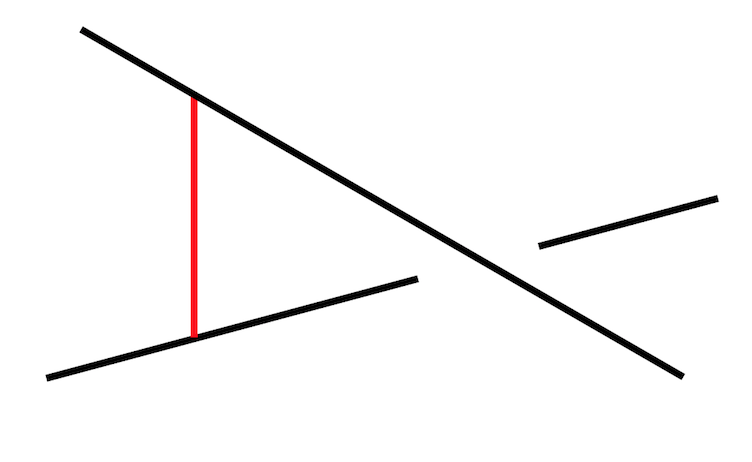
\includegraphics[width=4cm]{crossingArc.png}
%& 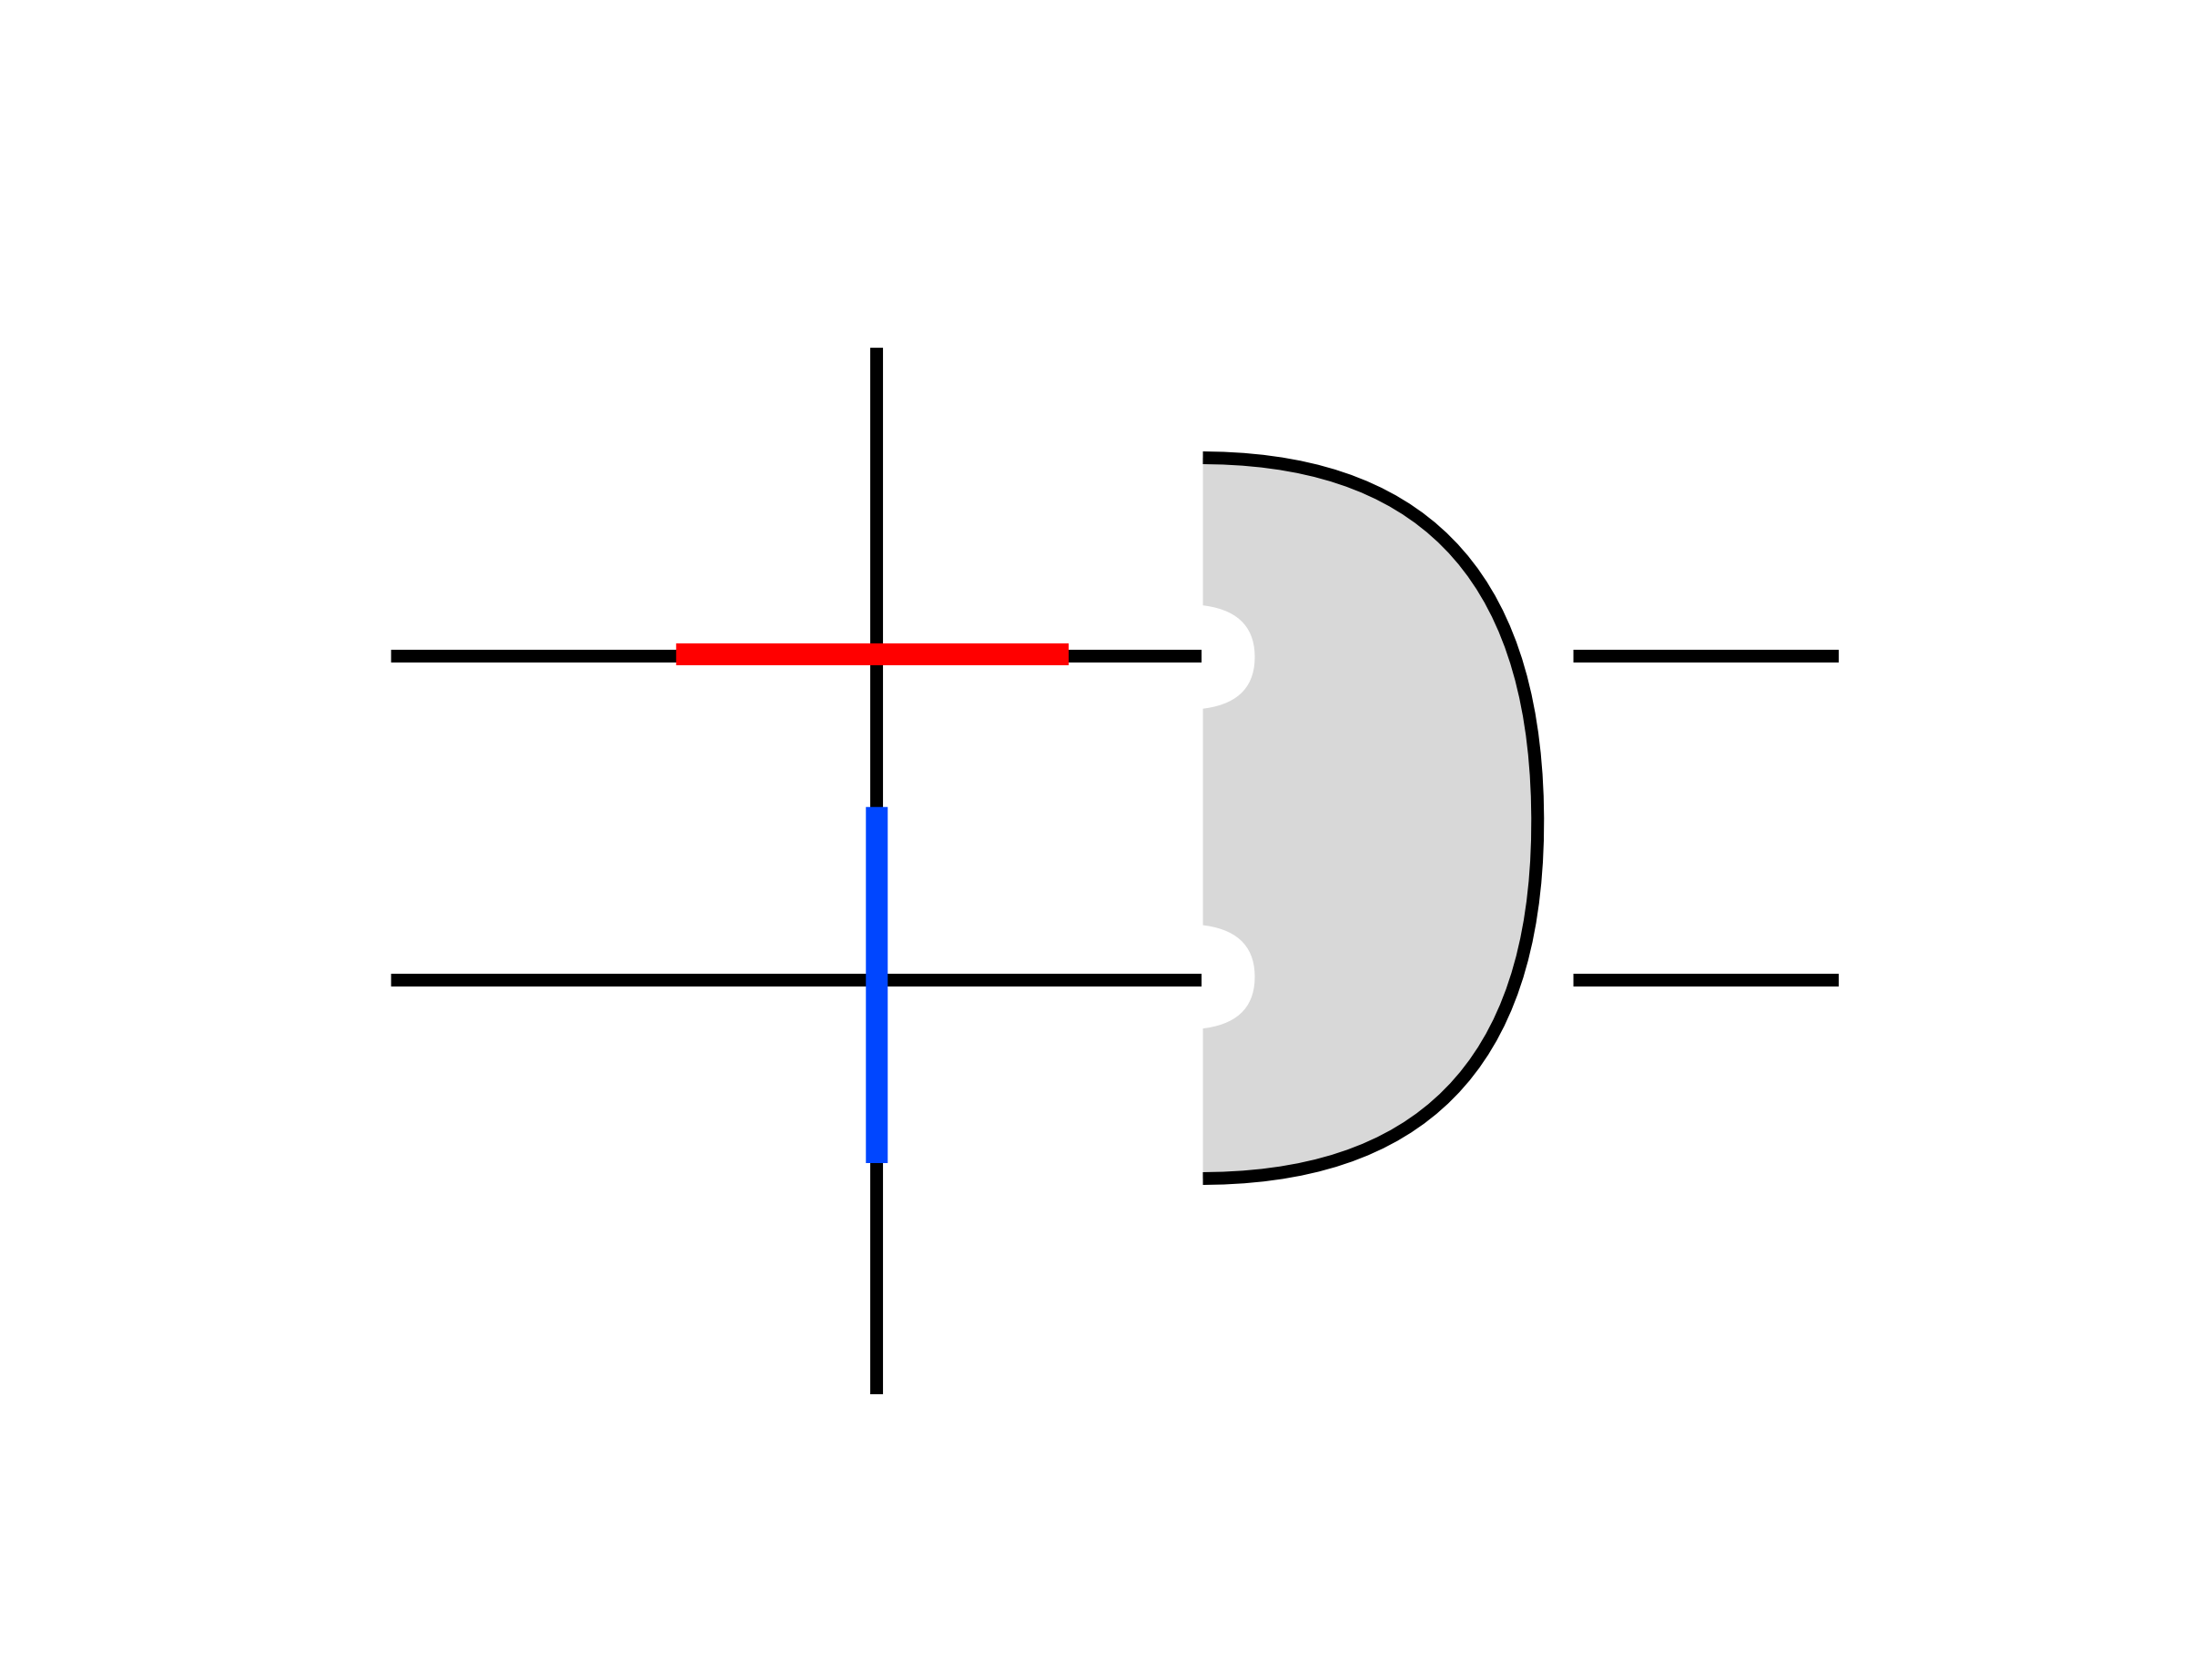
\includegraphics[width=5cm]{crossingPush.png}
%\\
%(a)
%& (b)
%\end{tabular}
%\caption{(a) The black strands are
%part of the link and the red strand is the crossing edge.
%(b) The blue and
%red edges represent the split crossing edges and the shaded half disk is bounded
%by the crossing circle} 
%\label{fig:crossingArc} 
\end{figure}


Next we construct the graph that will define the ``top'' torihedron.
We view the link from the point at infinity from the top end
($\torus \times \{1\}$) of the thickened torus.
At each crossing of $K$,
push the top strand towards the bottom strand,
splitting the crossing edge into two
identical edges and spreading them apart as in
\figref{f:crossing-edges}.
%Figure \ref{fig:crossingArc}.
% (b).
%We push the link
%components to infinity and stretch the crossing edge so that we have flattened
%the link onto $\torus \times \{0\}$ except for the crossing circles,
%which remains perpendicular to the projection plane. 
 

%Now place a disk on each crossing circle, so that the disk is bounded by
%the crossing circle.
Now for each crossing circle $c$, consider a spanning disk $B_c$;
$B_c$ intersects the projection plane $\torus \times \{0\}$
along the red segments in Figure \ref{fig:falGluings},
which consists of three edges.
We then cut $\torus \times I$ along $\torus \times \{0\}$ and
focus on the top half, $\torus \times [0,1)$.
(We will follow the same method on the
bottom half to obtain the second identical torihedron.)
The spanning disks we placed for each crossing circle are now cut in half
along the red segment.
Each half of the disk is now bounded by the
projection plane and the semi-circle arc of the crossing circle.
We push down on the crossing circle and split the half-disk into
two identical half-disks.
We then push the arc of each crossing circle to infinity,
collapsing them to ideal vertices.
We obtain two triangular faces which represent the half-disk which look like a
bow-tie as in Figure \ref{fig:falGluings} (a).
See Figures \ref{fig:step_one} to \ref{fig:top-bottom}
for an example.

\begin{figure}[ht]
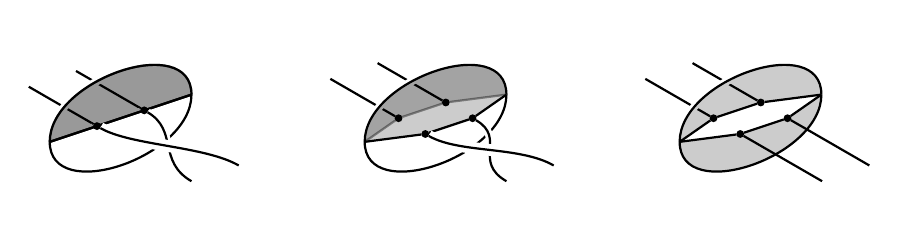
\begin{tikzpicture}
\begin{scope}[shift={(0,0)}]
\node[emptynode] (a) at (-0.9,-0.3) {};
\node[dotnode] (b) at (-0.3,-0.1) {};
\node[dotnode] (c) at (0.3,0.1) {};
\node[emptynode] (d) at (0.9,0.3) {};
%% two strands going out back
\draw (b) -- +(150:1cm);
\draw (c) -- +(150:1cm);
%% the ellipse; draw top arc, then fill, then bottom arc
\draw[thin_overline={1}] (a) -- (b) -- (c) -- (d)
	.. controls +(90:0.8cm) and +(90:0.8cm) .. (a);
\draw[fill, opacity=0.4] (a) -- (d)
	.. controls +(90:0.8cm) and +(90:0.8cm) .. (a);
\draw (a) -- (d)
	.. controls +(-90:0.8cm) and +(-90:0.8cm) .. (a);
%% two strands coming out front with twist
%\draw (b) -- +(-30:2cm); %\draw (c) -- +(-30:2cm);
\draw[thin_overline={1}] (c)
	.. controls +(-30:0.5cm) and +(150:0.5cm) .. (0.9,-0.8);
\draw[thin_overline={1.5}] (b)
	.. controls +(-30:0.5cm) and +(150:0.5cm) .. (1.5,-0.6);
\end{scope}
%%%%%%%%%%%%%%%%%%%%%%%%%%%%%%%%%%%%%%%%%%%%%%%%%%%%
\begin{scope}[shift={(4,0)}]
\node[emptynode] (a) at (-0.9,-0.3) {};
%\node[dotnode] (b) at (-0.3,-0.1) {};
%\node[dotnode] (c) at (0.3,0.1) {};
\node[dotnode] (e) at (-0.47,0) {};
\node[dotnode] (f) at (0.13,0.2) {};
\node[dotnode] (g) at (-0.13,-0.2) {};
\node[dotnode] (h) at (0.47,0) {};
\node[emptynode] (d) at (0.9,0.3) {};
%% two strands going out back
\draw (e) -- +(150:1cm);
\draw (f) -- +(150:1cm);
%% the ellipse; draw top arc, then fill, then bottom arc
\draw[thin_overline={1}] (d)
	.. controls +(90:0.8cm) and +(90:0.8cm) .. (a);
\fill[opacity=0.2] (a.center) -- (e.center) -- (f.center) -- (d.center)
	.. controls +(90:0.8cm) and +(90:0.8cm) .. cycle;
\fill[opacity=0.2] (a.center) -- (g.center) -- (h.center) -- (d.center)
	.. controls +(90:0.8cm) and +(90:0.8cm) .. cycle;
\draw (a) -- (g) -- (h) -- (d);
\draw[opacity=0.4] (a) -- (e) -- (f) -- (d);
\draw (d)
	.. controls +(-90:0.8cm) and +(-90:0.8cm) .. (a);
%% two strands coming out front with twist
%\draw (g) -- +(-30:2cm); \draw (h) -- +(-30:2cm);
\draw[thin_overline={1}] (h)
	.. controls +(-30:0.5cm) and +(150:0.5cm) .. (0.9,-0.8);
\draw[thin_overline={1.5}] (g)
	.. controls +(-30:0.5cm) and +(150:0.5cm) .. (1.5,-0.6);
\end{scope}
%%%%%%%%%%%%%%%%%%%%%%%%%%%%%%%%%%%%%%%%%%%%%%%%%%%%%
\begin{scope}[shift={(8,0)}]
\node[emptynode] (a) at (-0.9,-0.3) {};
%\node[dotnode] (b) at (-0.3,-0.1) {};
%\node[dotnode] (c) at (0.3,0.1) {};
\node[dotnode] (e) at (-0.47,0) {};
\node[dotnode] (f) at (0.13,0.2) {};
\node[dotnode] (g) at (-0.13,-0.2) {};
\node[dotnode] (h) at (0.47,0) {};
\node[emptynode] (d) at (0.9,0.3) {};
%% two strands going out back
\draw (e) -- +(150:1cm);
\draw (f) -- +(150:1cm);
%% the ellipse; draw top arc, then fill, then bottom arc
\draw[thin_overline={1}] (d)
	.. controls +(90:0.8cm) and +(90:0.8cm) .. (a);
\fill[opacity=0.2] (a.center) -- (e.center) -- (f.center) -- (d.center)
	.. controls +(90:0.8cm) and +(90:0.8cm) .. cycle;
\fill[opacity=0.2] (a.center) -- (g.center) -- (h.center) -- (d.center)
	.. controls +(-90:0.8cm) and +(-90:0.8cm) .. cycle;
\draw (a) -- (g) -- (h) -- (d);
\draw (a) -- (e) -- (f) -- (d);
\draw (d)
	.. controls +(-90:0.8cm) and +(-90:0.8cm) .. (a);
%% two strands coming out front with twist
\draw (g) -- +(-30:1.2cm); \draw (h) -- +(-30:1.2cm);
%\draw[thin_overline={1}] (h)
%	.. controls +(-30:0.5cm) and +(150:0.5cm) .. (0.9,-0.8);
%\draw[thin_overline={1}] (g)
%	.. controls +(-30:0.5cm) and +(150:0.5cm) .. (1.5,-0.6);
\end{scope}
\end{tikzpicture}


\caption{Removing half-twists from augmented twist-regions}
\label{f:cut-slice-flatten}
\end{figure}

\begin{figure}
\centering
\begin{tabular}{cc}
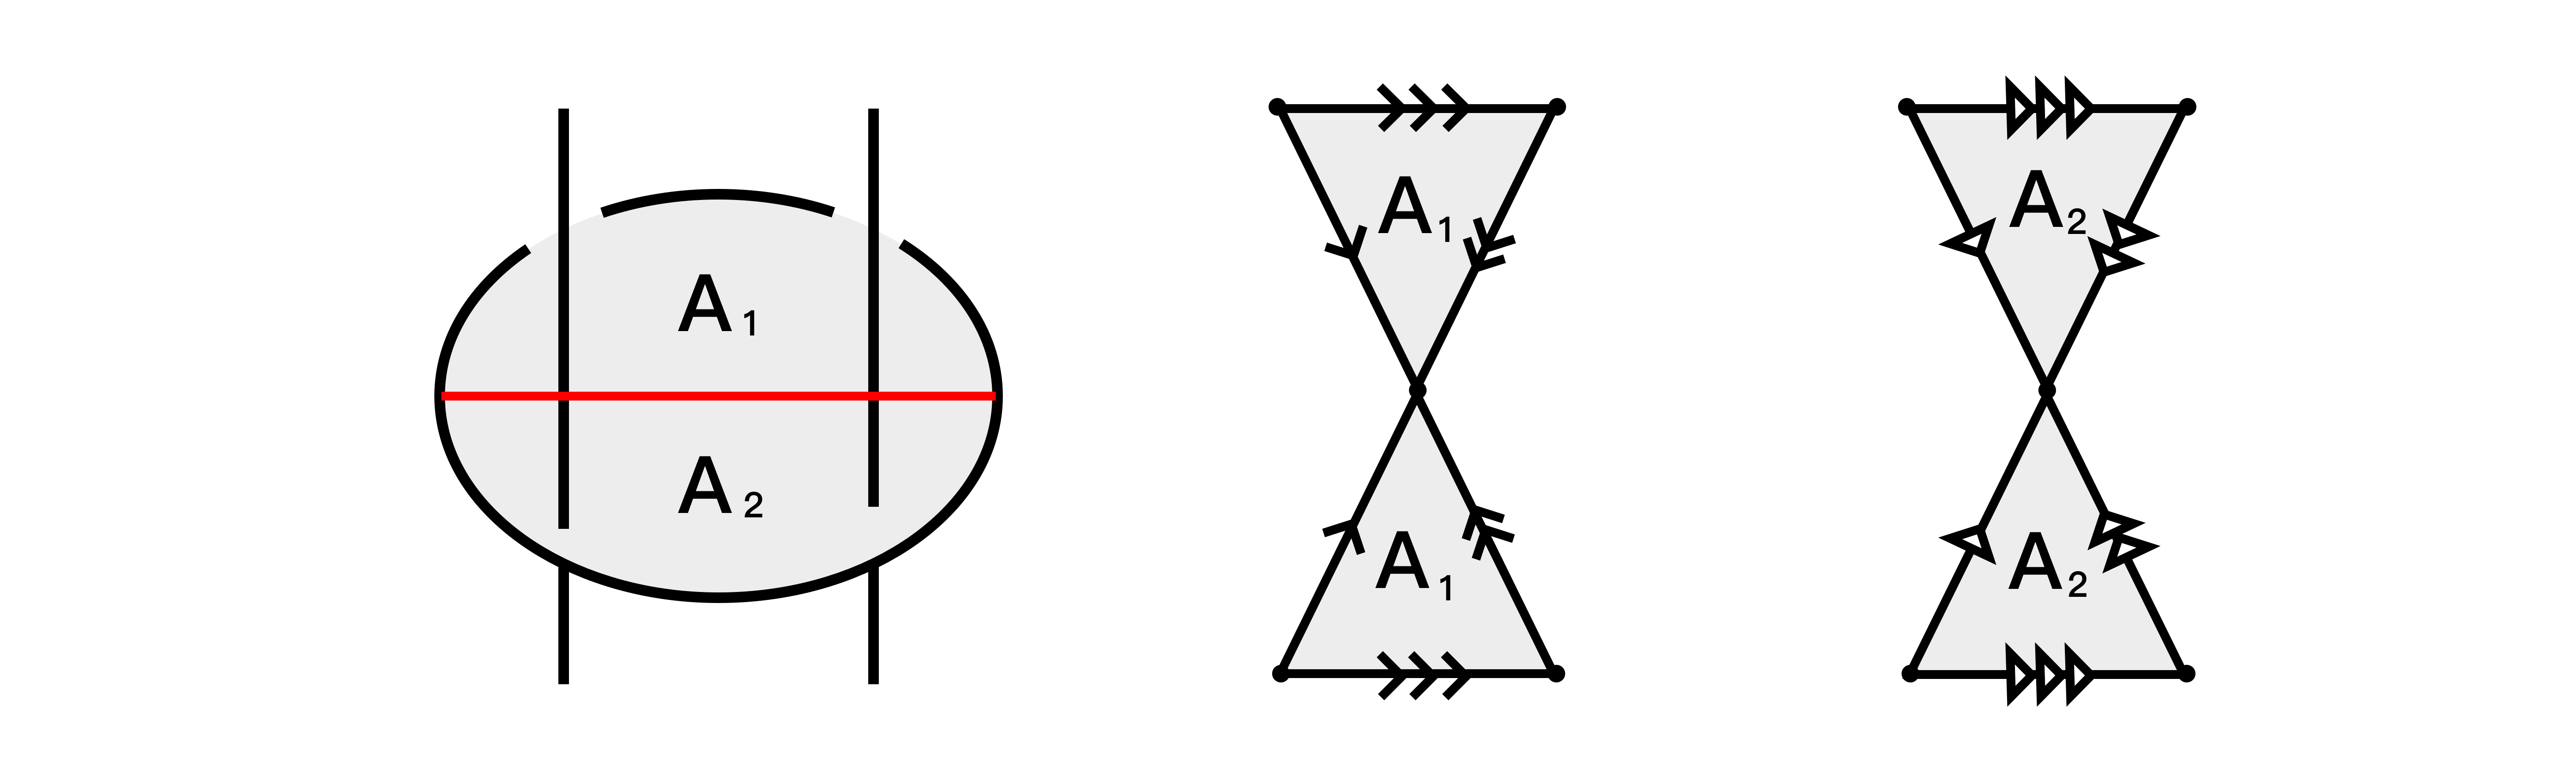
\includegraphics [width=8cm]{falGluing1.png}&
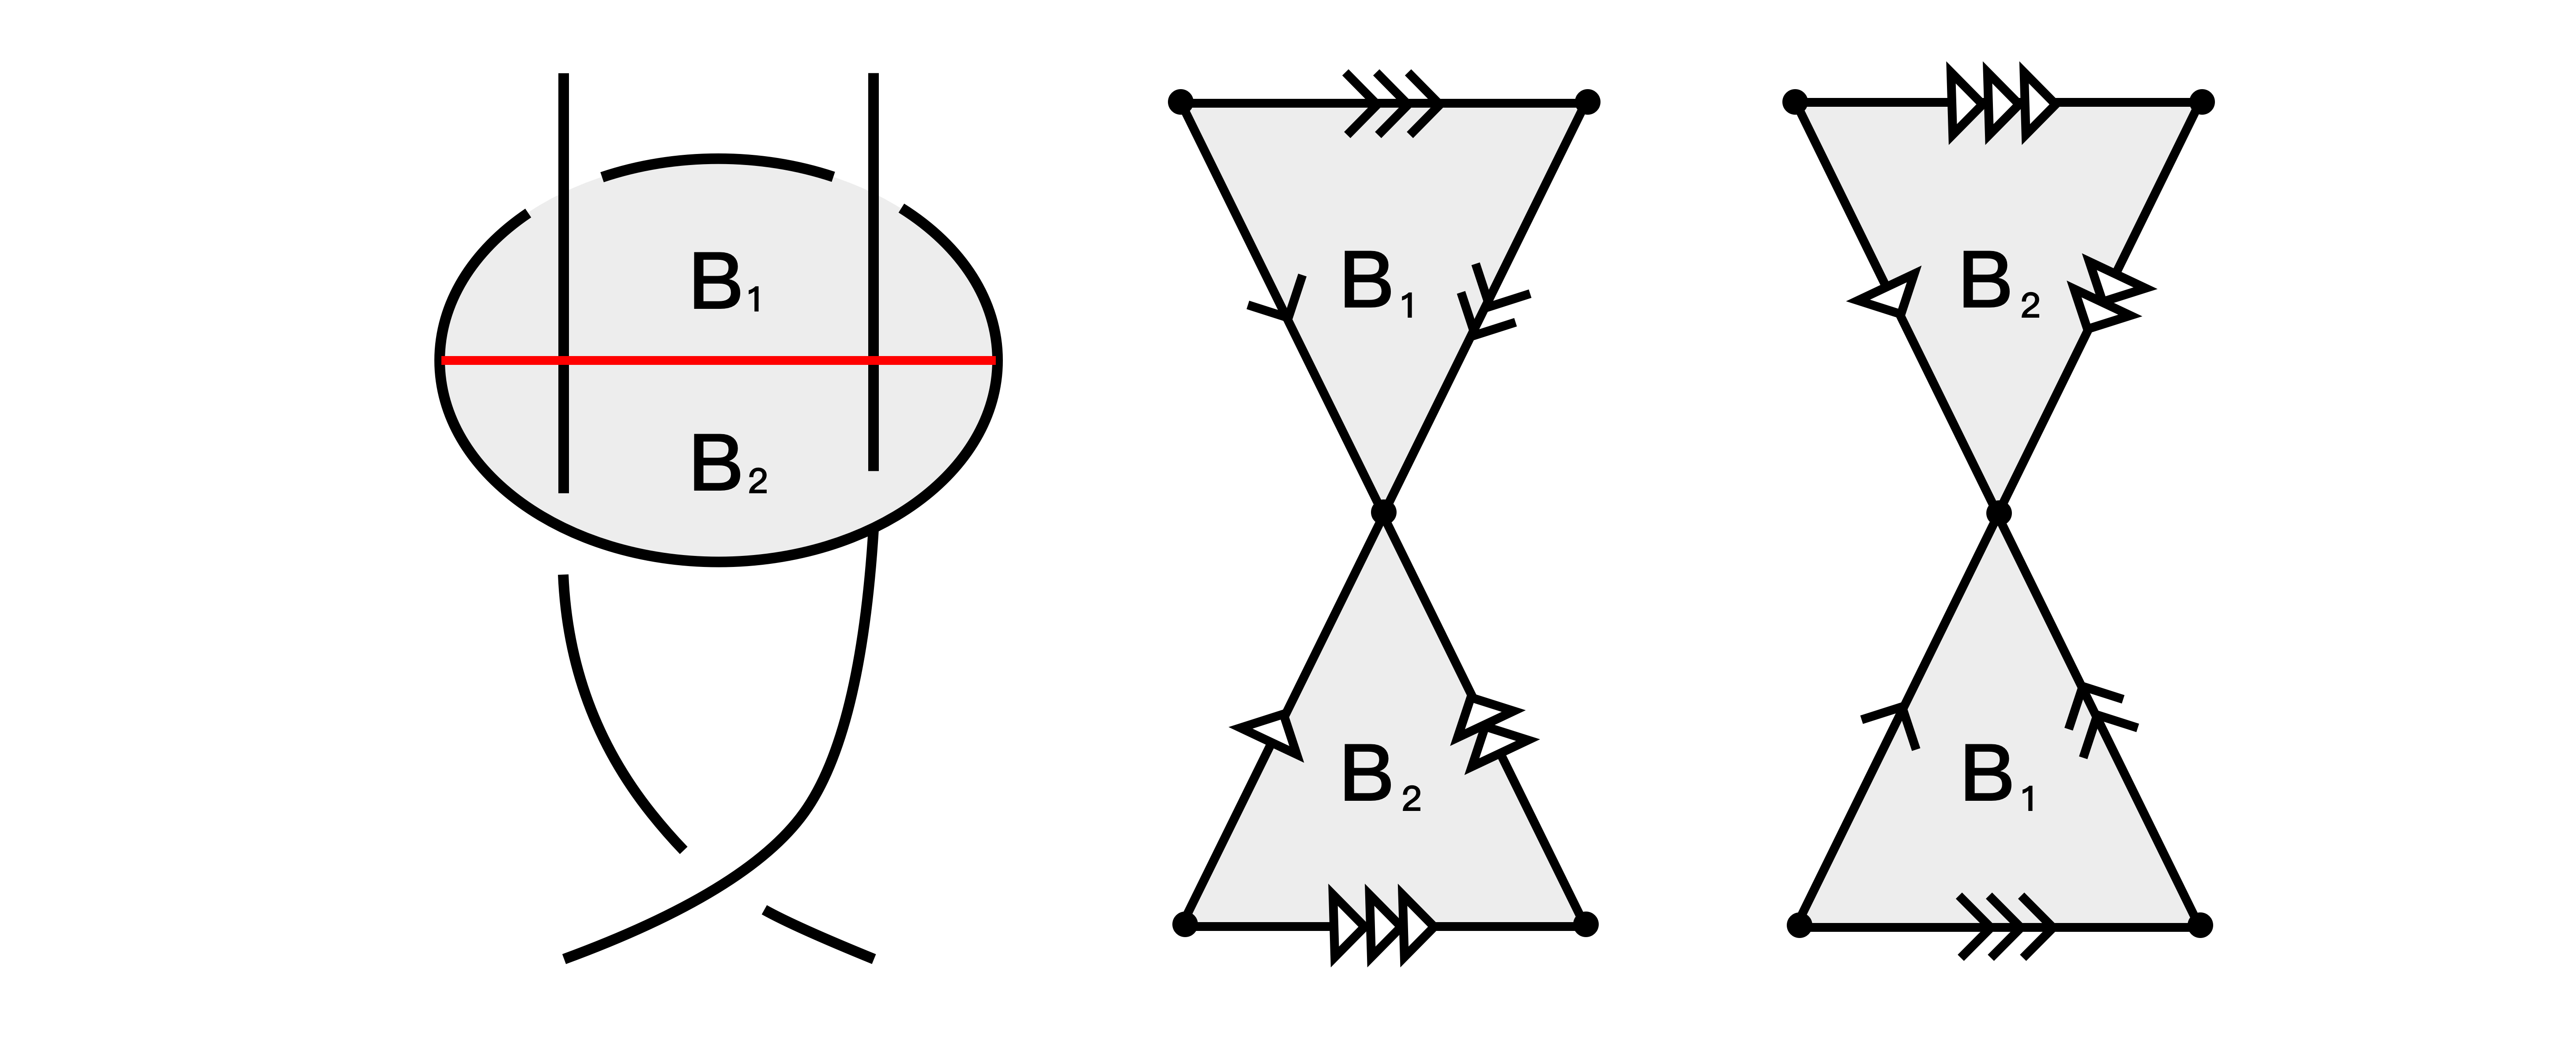
\includegraphics [width=7cm]{falGluing2.png}\\
(a)&(b)
\end{tabular}
\caption{(a) Gluing of bow-ties without half-twists
(b) Gluing with half-twists}
\label{fig:falGluings}
\end{figure}


The crossing edges and edges from spanning disks of crossing circles
form the graph of the top ideal torihedron.
It is not hard to see that this graph is $\Gamma_T(L)$.
We repeat similar steps for the bottom half of $\torus \times I$,
$\torus \times (-1,0]$
(note we should be pushing the bottom strands up towards the top strand).
It is also easy to see that this graph is $\Gamma_B(L)$
(from the same perspective, not from the perspective of the bottom end
$\torus \times \{-1\}$).
Thus we get two ideal torihedra.
%The graph of each will come from
%crossing edges and edges from spanning disks of crossing circles.


We obtain the complement of $L$ by gluing the two torihedra with the gluing
information given by identifying crossing edges and triangles of the bow-tie.
As observed before, the non-bow-tie faces of $\Gamma_T(L),\Gamma_B(L)$
naturally pair up, and we glue them accordingly
(there is a ``$2\pi/n$'' twist when gluing these faces,
where $n$ is the number of sides of each face as in Figure
\ref{fig:top-bottom} clockwise or counterclockwise).
The bow-tie triangular faces are glued up according to
\figref{fig:falGluings} (a).
%We glue the faces of the torihedra which do not correspond to a bow-tie with a
%$2\pi/n$ twist where $n$ is the number of sides of each face as in Figure
%\ref{fig:top-bottom} clockwise or counterclockwise.


Now, if $L$ has half-twists,
we apply the constructions above to $L'$,
which is the link obtained from $L$ by removing all half-twists
(replacing them with parallel strands).
The complement of $L$ is again obtained by
gluing the torihedra together all the same,
except that at the bow-ties coming from twist regions with a half-twist,
they are glued as in Figure \ref{fig:falGluings} (b).
%we decompose the complement of the link the same way
%(as if there are no half twists)
%but we identify the two bow-ties as in Figure \ref{fig:falGluings} (b).
%Finally,


%%For future reference, we will denote the graph for the top and bottom
%%torihedra by $\Gamma_T(L)$ and $\Gamma_B(L)$, respectively,
%%where both graphs are viewed from the cone point of the top torihedron
%%$\torus \times \{1\}$.
%%Note that if $L = K$ is the non-augmented link,
%%$\Gamma_T(L)$ is simply the link projection of $K$,
%%and in fact $\Gamma_T(K) = \Gamma_B(K)$.
\end{proof}




%%%%%%%%%%%%%%%%%%%%%%%%%%%%
The Figures \ref{fig:step_one} to \ref{fig:top-bottom}
depict an example which decomposes the link (C) of Figure
\ref{fig:Augmentations}. 


\begin{figure}[h] 
\centering
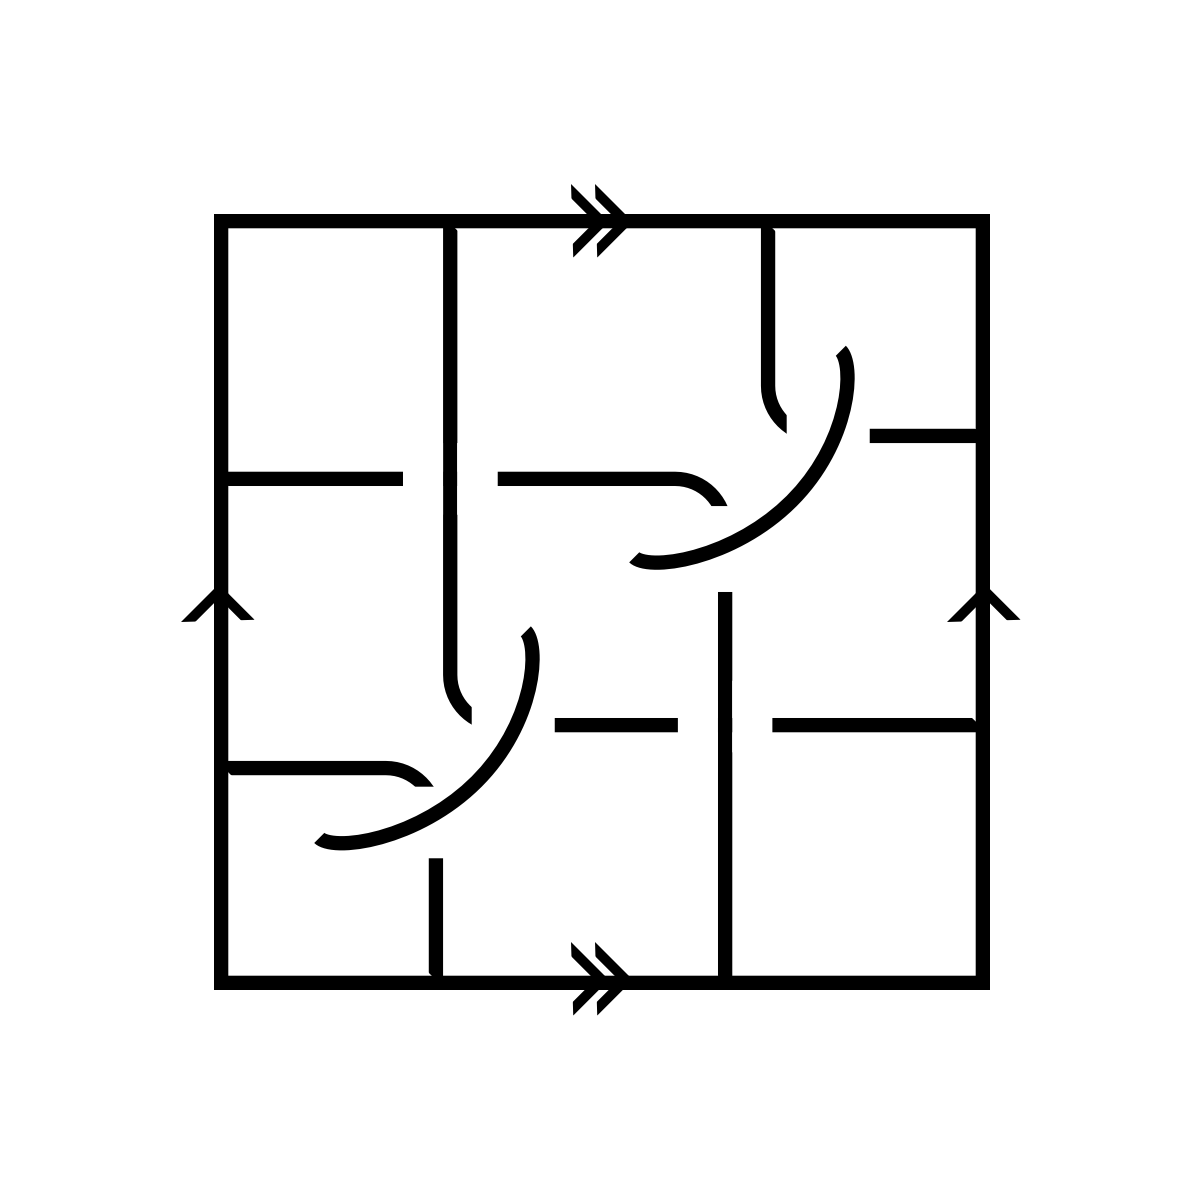
\includegraphics[height=3cm]{fig-3.png}
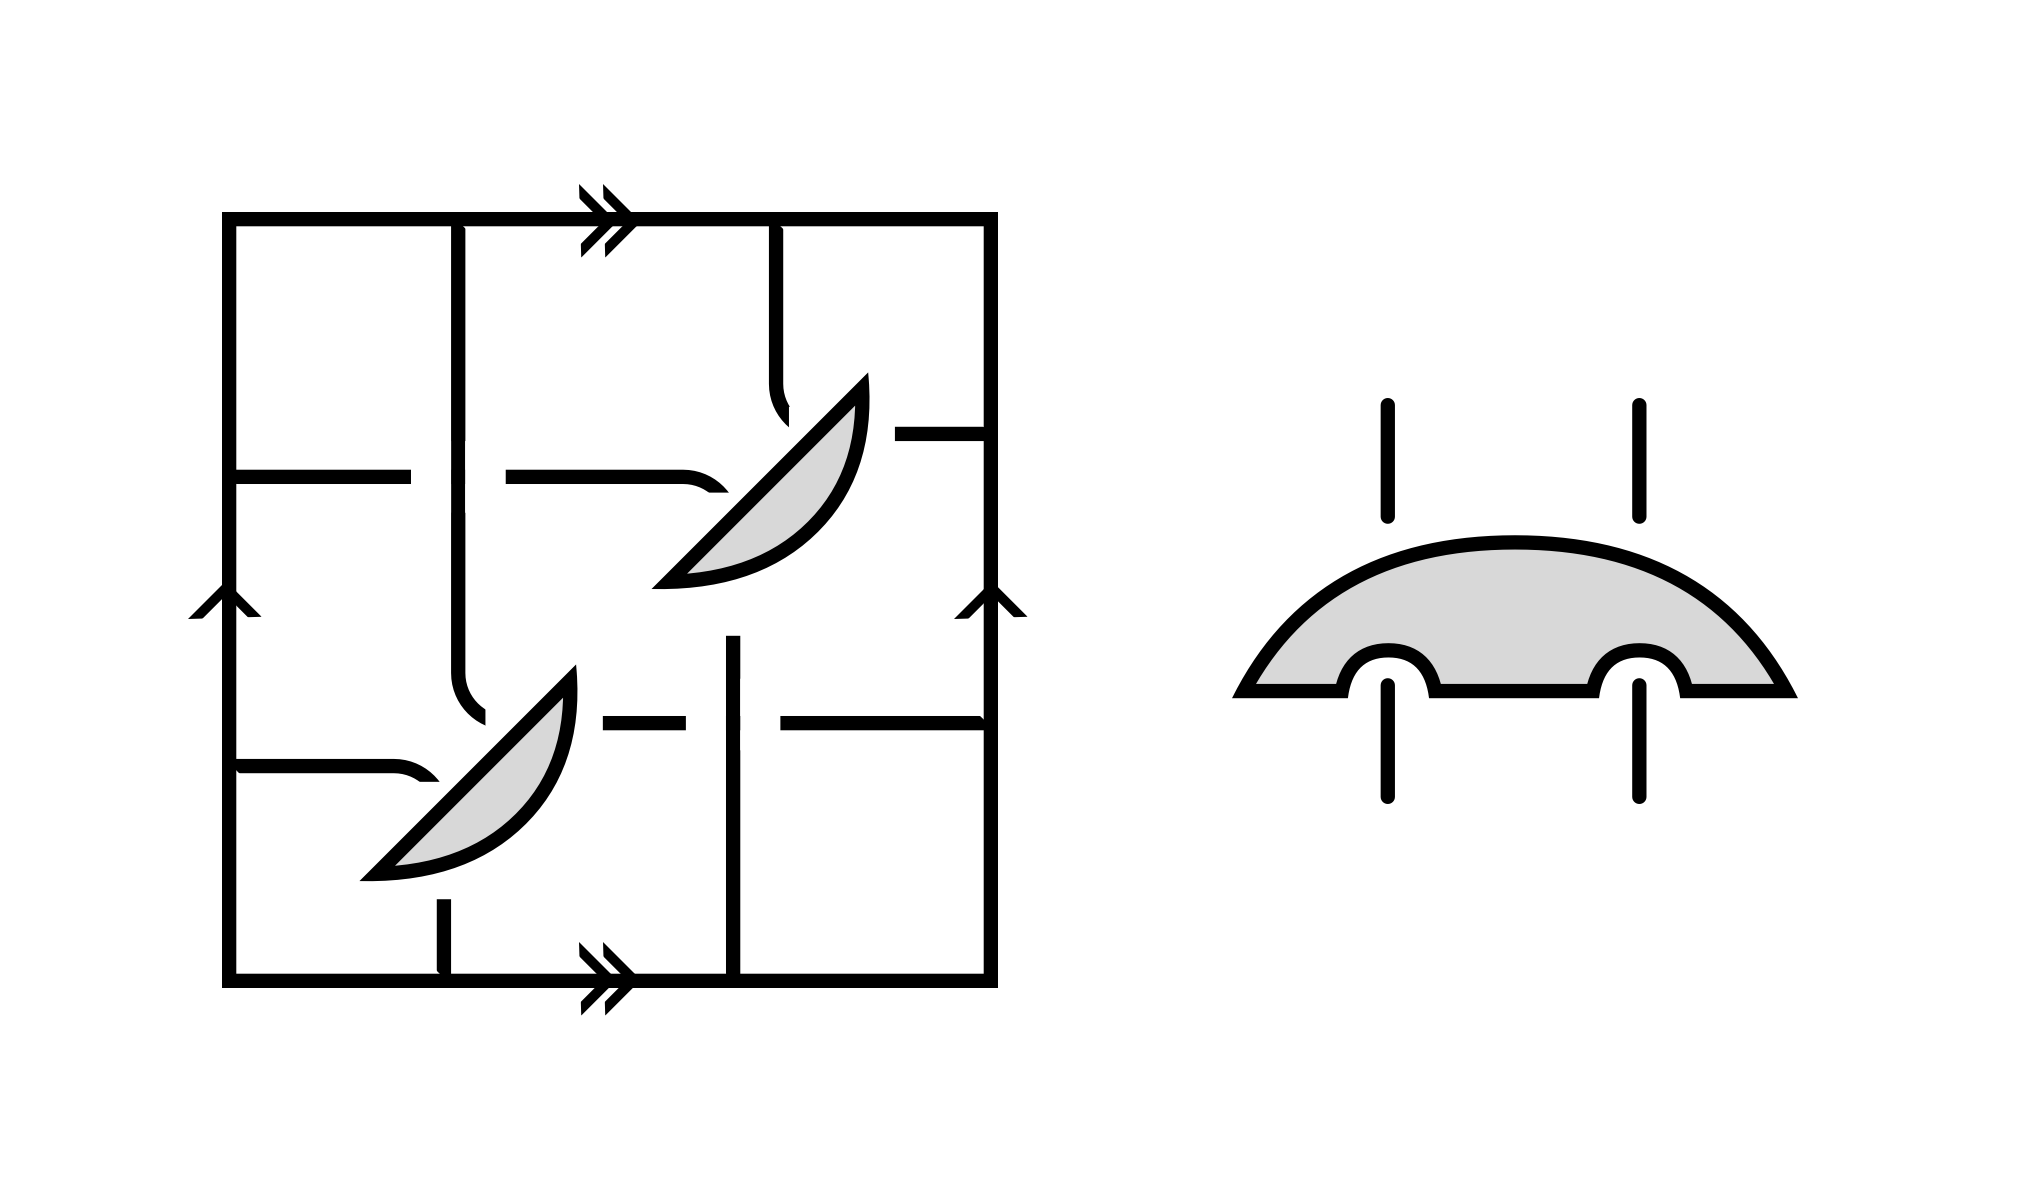
\includegraphics[height=3cm]{fig-4.png}
	\caption{Each crossing circle bounds a twice-punctured disk}
	\label{fig:step_one}
\end{figure}
 
%\vspace{-0.5cm} 
\begin{figure}[h] 
\centering 
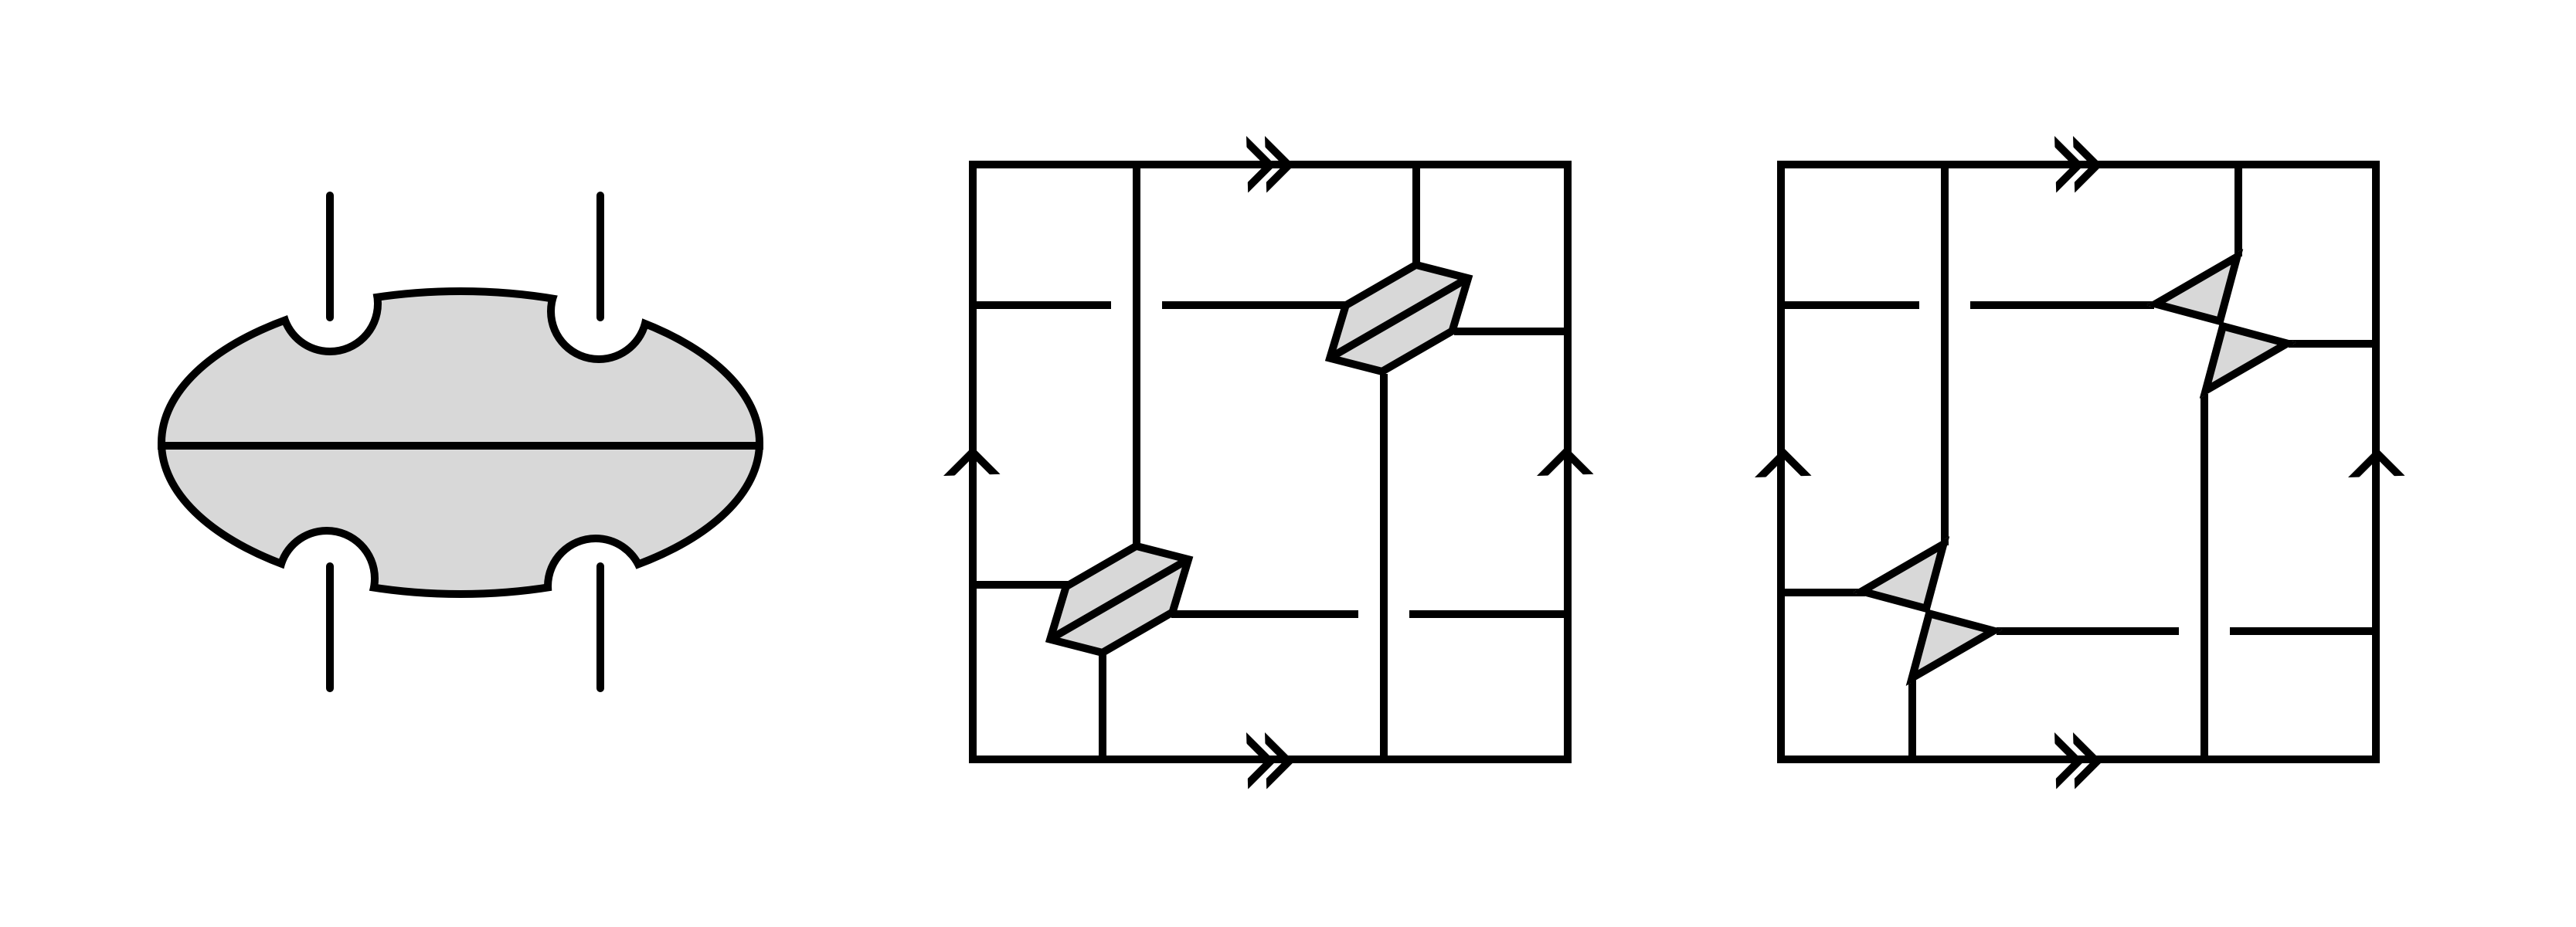
\includegraphics[height=3cm]{fig-5.png} 
	\caption{We split the disk and collapse the arc of each
 crossing circle to ideal vertices}
	\label{fig:step_two}
\end{figure}


\begin{figure}[h] 
\centering 
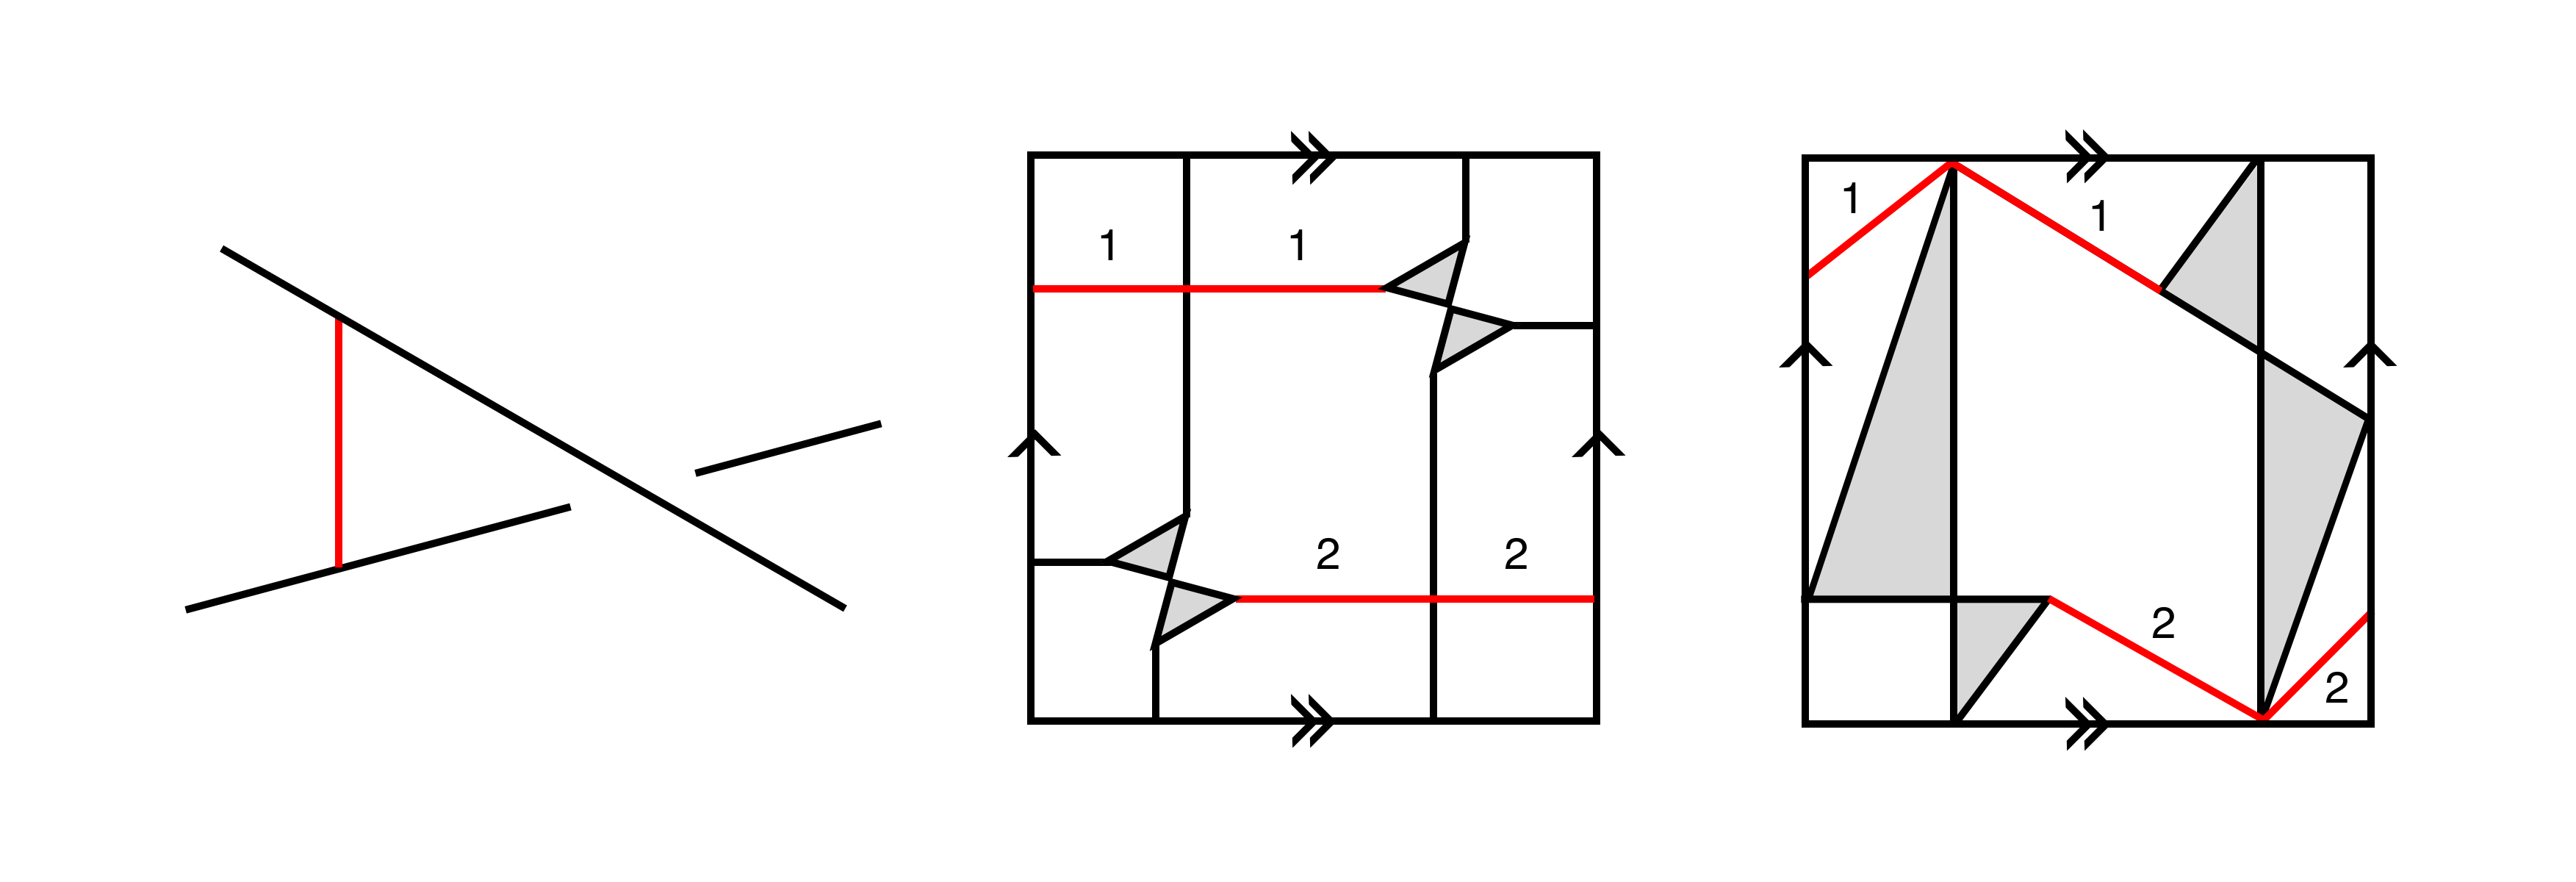
\includegraphics[height=3cm]{fig-6.png} 
\caption{Left: The crossing arc is the edge in red.
Middle: Picture of splitting the crossing edge.
Right: The link components are pushed off to infinity.}
	\label{fig:step_three}
\end{figure}

\begin{figure}[h] 
\centering 
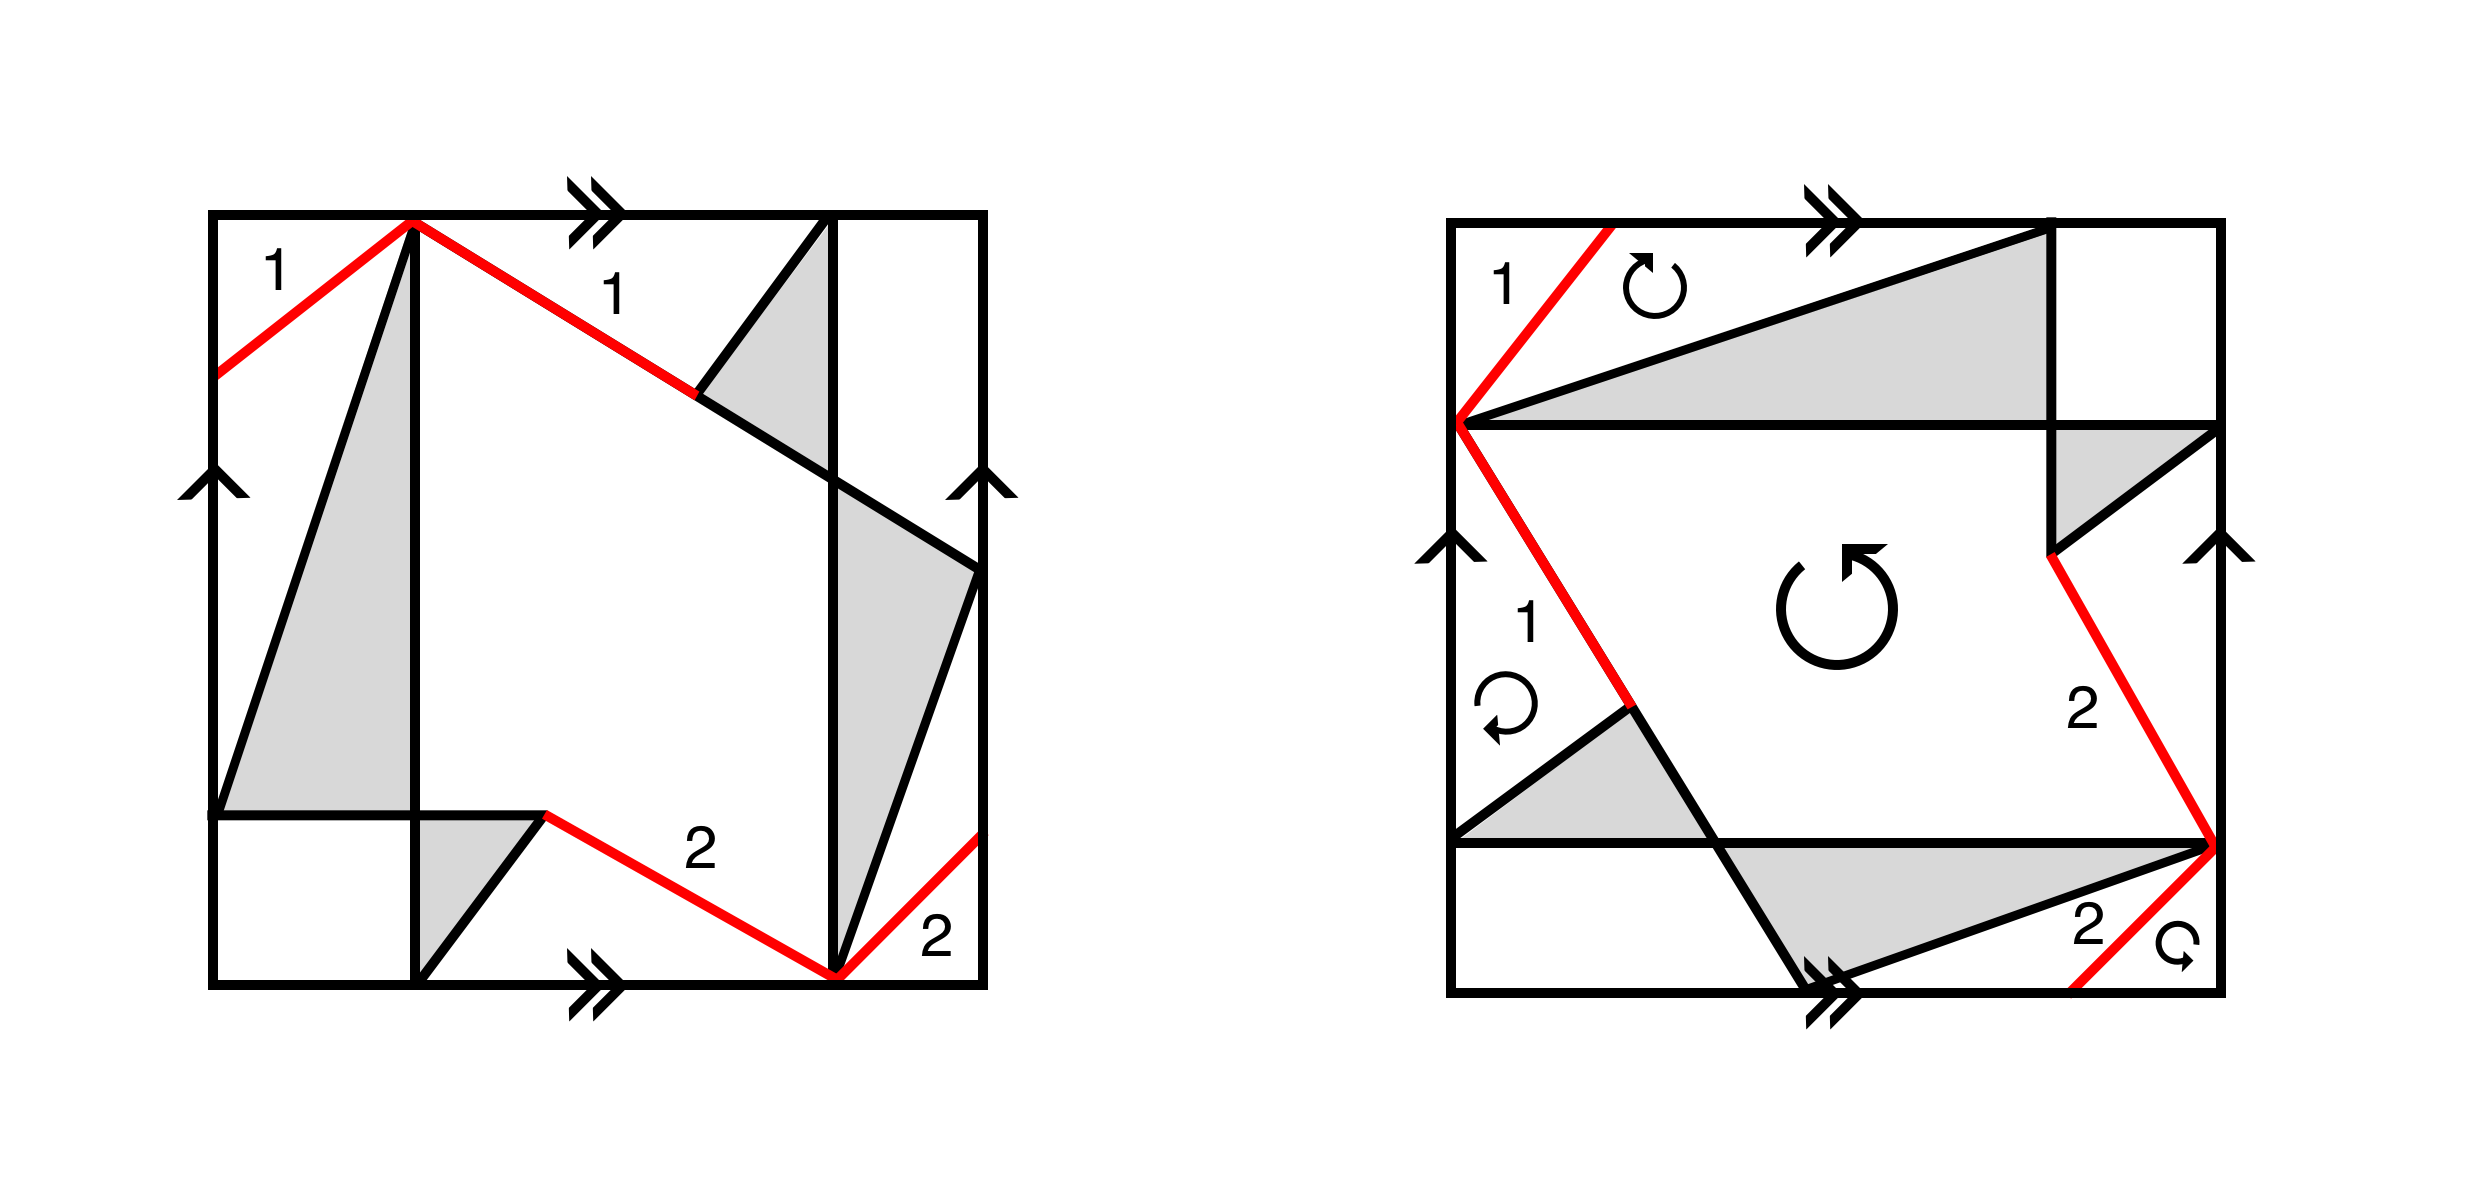
\includegraphics[height=3cm]{top-bottom.png} 
	\caption{Left: The top torihedron.
	Right: The bottom torihdron with rotation indicating face gluing;
	TODO shouldn't it be rotating other way?} 
\label{fig:top-bottom}
\end{figure}


\begin{remark}
We note that our main \thmref{t:auglink_hyp}
requires that all non-trivial twist regions be augmented,
but \prpref{p:tori_decomp} does not require it.
\label{r:unnecessary-augment-bigon}
\end{remark}


\begin{definition}
An \emph{angled torihedron} $(\sT, \theta_\bullet^*)$
is a torihedron $\sT$ with
an assignment of an \emph{interior dihedral angle}
$\theta_e^* \in [0,\pi]$ to each edge $e$ of $G(\sT)$
such that for each vertex $v \in G(\sT)$,
$\sum_{e \ni v} \theta_e^* = (\deg(v) - 2)\pi$.
We also denote $\theta_e = \pi - \theta_e^*$,
so $\sum_{e \ni v} \theta_e = 2\pi$;
we refer to $\theta_e$ as the \emph{exterior dihedral angle}.
%and $\theta_e^*$ as the interior angle. 
For brevity, we write dihedral angle to mean 
interior dihedral angle.  


We say $(\sT, \theta_\bullet^*)$ is \emph{degenerate}
if $\theta_e^* = 0$ for some edge;
we say it is \emph{non-degenerate} otherwise.
\end{definition}


One may ask for the pyramidal decomposition of a torihedron
to ``respect" angles. The following definitions,
in particular an ``angle splitting'', make sense of this.

\begin{define}
An \emph{angled ideal tetrahedron} is an ideal tetrahedron
with an assignment of an
interior dihedral angle $\theta_e^*$ to each edge $e$, such that
\begin{itemize}
\item each dihedral angle is in $[0, \pi]$;
\item for each tetrahedron, opposite edges have equal dihedral angles;
\item the three distinct interior angles at edges incident to one vertex sum to $\pi$.
\end{itemize}

We say an angled ideal tetrahedron is \emph{degenerate} if
one dihedral angle is 0; we say it is \emph{non-degenerate} otherwise.
\end{define}


\begin{define}
A \emph{base-angled ideal pyramid}
is a pyramid whose base is an $n$-gon, $n \geq 3$,
and each boundary edge $e_i$ of the base face is assigned a dihedral angle
$\alpha_i \geq 0$ such that their sum is $\sum \alpha_i = \pi$.
The vertical edge $e_i'$ that meets $e_i$ and $e_{i+1}$
is automatically assigned the dihedral angle $\pi - \alpha_i - \alpha_{i+1}$.


We say a base-angled ideal pyramid is \emph{degenerate} if
$\alpha_i = 0$ for some $i$; we say it is \emph{non-degenerate} otherwise.
\end{define}


Clearly, the dihedral angles of an ideal hyperbolic pyramid
make it a base-angled ideal pyramid
(with $\alpha_i = \vphi_{e_i}$);
it is not hard to see that the converse is true:
simply consider a circumsribed polygon such that the side $e_i$
subtends an angle of $2\alpha_i$ at the center,
and take the ideal hyperbolic pyramid over it in upper-half space.
Also, an angled ideal tetrahedron is simply a base-angled ideal pyramid
with base a triangle, and with no preferred face.

\begin{definition}
%TODO: this definition should come after base-angled pyramid
An \emph{angle-splitting} of an angled torihedron $(\sT,\theta_\bullet^*)$
is an assignment of an angle $\vphi_{\vec{e}}$ to each
oriented edge $\vec{e}$, such that

\begin{itemize}
\item for each edge $e$,
$\theta_e^* = \vphi_{\vec{e}} + \vphi_{\cev{e}}$,
where $\cev{e}$ is the opposite orientation on $e$,
\item for each face $f$,
$\sum_{\vec{e} \in \del f} \vphi_{\vec{e}} = \pi$,
where $\vec{e} \in \del f$ is the edge in the boundary of $f$
taken with outward-orientation
(see Convention \ref{cvn:ornt-edge}).
\end{itemize}


Equivalently, an angle-splitting is a decomposition of
$\sT$ into base-angled pyramids,
one for each face $F$ of $G(\sT)$, such that
the interior dihedral of the edge $\vec{e} \in \del F$
is $\vphi_{\vec{e}}$.
%for each boundary edge $e$ of $\sT$,
%the dihedral angles from the two adjacent pyramids
%add to $\theta_e^*$.


We also say that $\vphi_\bullet$ is an angle-splitting
of the edge-labeled graph $(G(\sT), \theta_\bullet^*)$.


We say that an angle-splitting is \emph{degenerate}
if $\vphi_{\vec{e}} = 0$ for some oriented edge $\vec{e}$;
it is \emph{non-degenerate} otherwise.
\end{definition}


\begin{convention}
The outward-orientation on the boundary of a face
is the orientation such that the face is to the left of the boundary.
An assignment/label on an oriented edge $\vec{e}$
(for example, $\vphi_{\vec{e}}$)
will usually be drawn to the left of that edge.
\label{cvn:ornt-edge}
\end{convention}


\begin{remark}
These $\theta$'s are the same as the $\theta$'s in
\cite{BandS},
and angle-splittings $\vphi_\bullet$'s
are the same as their ``coherent angle system''.
\end{remark}


%TODO remark on what splitting means in terms of ideal hyperbolic

\begin{lemma}
\label{l:pyramid_decomp}
%Let $P_n$ be an ideal pyramid whose base is an $n$-gon and suppose,
%\begin{itemize}
%\item each boundary edge of the base face is assigned a dihedral angle $\alpha_i$ such that for adjacent edges, $\alpha_i + \alpha_{i+1} < \pi$;
%\item we are given a decomposition of the base face into triangles by adding new edges. 
%\end{itemize}
Let $P_n$ be a base-angled ideal pyramid, and suppose we are given a
decomposition of the base face into triangles by adding new edges.  One gets an
obvious corresponding triangulation of $P_n$, where a new face is added for each
new edge. Then there is an assignment of a dihedral angle to each edge of each
ideal tetrahedron in this triangulation such that
\begin{itemize}
\item each tetrahedron is an angled ideal tetrahedron;
\item the sum of dihedral angles around each new edge is $\pi$;
\item the dihedral angles of the edges of the original base face are the same as
	before.
\end{itemize} 
Moreover, if $P_n$ is non-degenerate,
then the resulting angled tetrahedra are also non-degenerate.
\end{lemma}

\begin{proof}
Induct on $n$; there is nothing to prove for the base case $n=3$.


The proof is essentially given in Figure \ref{f:ideal_pyramid_arg}.
We spell it out here in words.


\begin{figure}
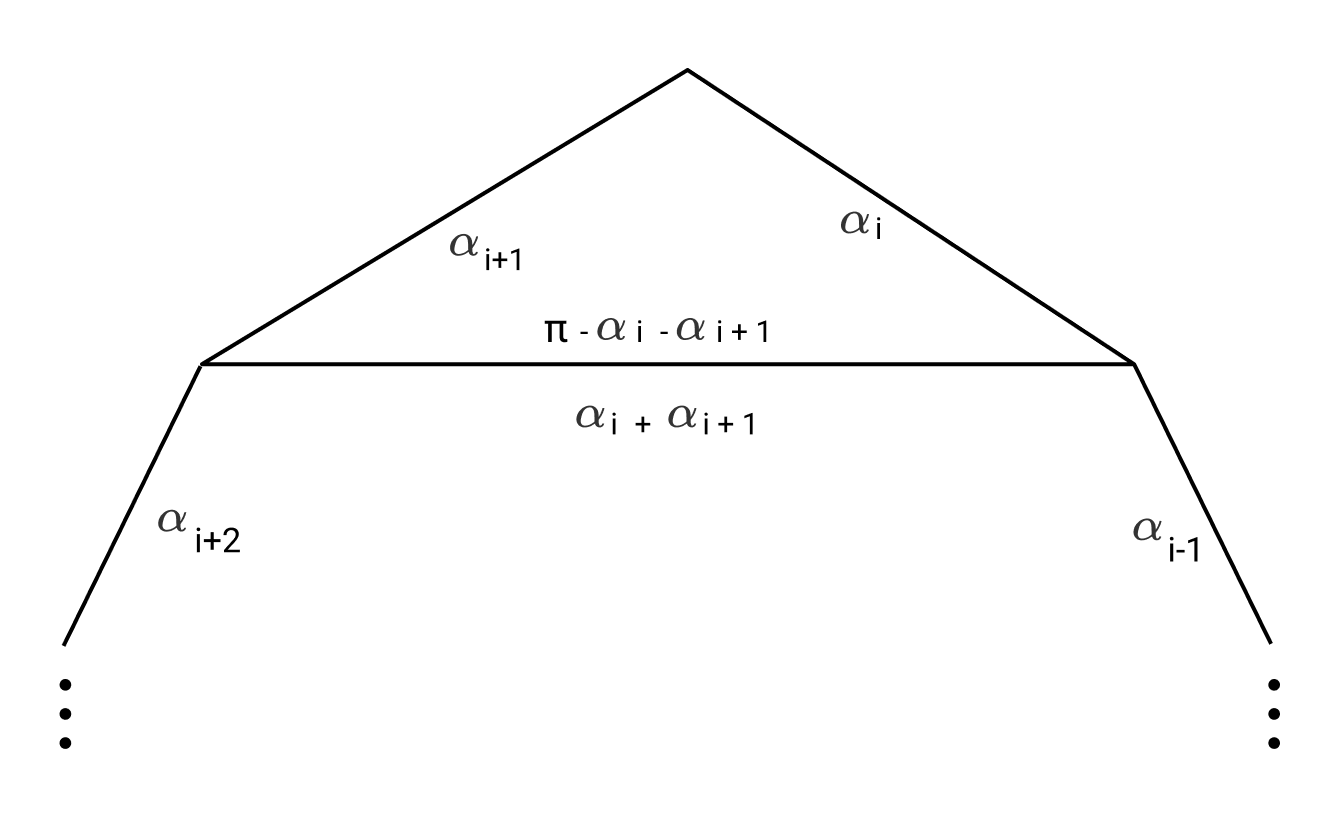
\includegraphics[height=5cm]{more_pictures/angle_split.png}
\caption{Angle-splitting on a polygonal face of the graph}
\label{f:ideal_pyramid_arg}
\end{figure}


Suppose the edges are labeled $e_i$, for an edge
which goes between vertices $v_i$ and $v_{i+1}$,
and suppose $e_i$ is assigned dihedral angle $\alpha_i$.
Let $e'$ be a new edge addeed to the base face of $P_n$
such that it separates the base face into a triangle and
an $(n-1)$-gon;
suppose the sides of the triangle are
$e_i, e_{i+1}$, and $e'$.
The new face corresponding to $e'$ separates $P_n$ into
an ideal tetrahedron $T$ and an ideal pyramid $P_{n-1}$.
We assign the dihedral angle of $\pi - \alpha_i - \alpha_{i+1}$
to $e'$ in $T$, and assign $\alpha_i + \alpha_{i+1}$ to $e'$ in $P_{n-1}$.
Clearly the sum of dihedral angles condition is satisfied
in $T$ and $P_{n-1}$.
It remains to check that the dihedral angles assigned to the vertical (non-base)
edges are correct.
For the vertical edge associated to $v_j$ for $j \neq i, i+2$,
there is nothing to check;
for $j = i$, the dihedral angles are
$\pi - \alpha_i - (\pi - \alpha_i - \alpha_{i-1})$
in $T$ and $\pi - \alpha_{i-1} - (\alpha_i + \alpha_{i+1})$ in $P_{n-1}$,
which sum to $\pi - \alpha_i - \alpha_{i+1}$;
it is similar for $j = i+2$.


Non-degeneracy of the resulting angled tetrahedra
follows easily from the observation that the angles
assigned to each side of a new edge is simply the sum
of the angles of original edges on the other side.
\end{proof}


%%%%%%%%%%%%%%%%%%%%%%%%%%%%%%%%%%%%%%%%%%%%%%%%%%%%%%%%%%%
\section{Hyperbolicity of Augmented Links}
\label{s:hyperbolicity}
Thurston introduced a method for finding the
unique complete hyperbolic metric for a given 3-manifold $M$
with boundary consisting of tori \cite{Thurston}. 
%The idea
%was to triangulate the interior of $M$ into ideal tetrahedra and give those
%tetrahedra hyperbolic shapes (called shape parameters) that glue up coherently
%in $M$. The shape parameter of a tetrahedron is described by the cross-ratio of
%its four vertices on the sphere at infinity. 
Thurston wrote down a system of gluing and consistency equations
which can be translated to equations involving
angles for a triangulation of $M$ whose solutions correspond to the
complete hyperbolic metric on the interior of $M$.
Casson and Rivin separated Thurston's
gluing equations into a linear and non-linear part \cite{Casson-Rivin}.
Angle structures are solutions to the linear part of
Thurston's gluing equations;
we will use them to attain hyperbolicity of complements
of augmented links in the thickened torus.


\begin{define}
Let $M$ be an orientable 3-manifold with boundary consisting of tori. An angle
structure on an ideal triangulation $\tau$ of $M$ is an assignment of a dihedral
angle to each edge of each tetrahedron, such that
\begin{itemize}
\item each tetrahedron is a non-degenerate angled ideal tetrahedron,
\item around each edge of $\tau$, the dihedral angles sum to $2\pi$.
\end{itemize}
\end{define}

%\cite{TODO: find rivin's paper? should be in here https://arxiv.org/pdf/1004.0440.pdf}


\begin{theorem}\cite[Theorem 1.1]{FG-angles}
Let $M$ be a 3-manifold with a triangulation that admits an angle structure.
Then $M$ is hyperbolic.
\end{theorem}


For a hyperbolic link $K$ in $\torus \times I$, we show
that the link $L$ obtained from augmenting $K$ is hyperbolic.
The idea is to start with a graph from the torihedral decomposition
of the link $K$ which will give us a graph on each torihedron with an angle
assignment of $\pi/2$ to each edge \cite{CKP2}.
By \prpref{p:tori_decomp},
there is a torihedral decomposition of the complement of the augmented link $L$.
Using those angles from $K$,
we then assign new angles locally to edges of torihedra from a torihedral 
decomposition of $L$
and decompose them into base-angled pyramids which can be decomposed 
into tetrahedra, thus obtaining an angle structure on a triangulation.




We need the following theorem,
adapted from \cite[Theorem 4]{BandS},
specialized to genus 1 surfaces:


\begin{theorem}{\cite[Theorem 4]{BandS}}
Let $\Gamma = (V,E)$ be a graph on the torus,
and let $\check{\Gamma} = (F,\check{E})$ be the dual graph,
with $\check{E}$ being naturally identified with $E$.
%Let $\theta_\bullet \in (0,\pi)^E$
Let $f \in (0,\pi)^E$
be a function on the set of edges $E$
that sums to $2\pi$ around each vertex of $V$;
let $f^*(e) = \pi - f(e)$.


There exists a non-degenerate
%angle-splitting of $(\Gamma,\theta_\bullet)$
angle-splitting of $(\Gamma,f^*)$
if and only if the following is satisfied:

\begin{quotation}
Suppose we cut the torus along a subset of edges in the dual graph
$\check{\Gamma}$, obtaining one or more pieces;
Then for any piece that is a disc,
the sum of $f$ over the edges in the boundary
of the piece is at least $2\pi$,
with equality if and only if the piece
contains exactly one vertex of $\Gamma$.
\end{quotation}

\label{t:bs-thm4}
\end{theorem}

The original theorem \cite[Theorem 4]{BandS}
proves that a circle pattern combinatorially equivalent to $\Gamma$
exists; a circle pattern naturally yields
an angle-splitting (which they call a coherent angle system).


\begin{theorem}
\label{t:auglink_hyp}
Let $K$ be a weakly prime, alternating link
in the thickened torus
whose diagram is cellular and has no bigons.
Let $L$ be a link obtained from augmenting $K$.
Then $L$ is hyperbolic.


More generally, if $K$ is as above with a twist-reduced diagram
containing bigons,
and $L$ is obtained by augmenting $K$
such that every twist region with at least one bigon is augmented,
%(and possibly other crossings),
then $L$ is hyperbolic.
\end{theorem}

\begin{proof}
%Let us first consider the case when $K$ did not have bigons.
By \prpref{p:tori_decomp}, $\toruscomp{L}$ can be
obtained by gluing two torihedra $\sT_T(L),\sT_B(L)$
with graphs $\Gamma_T(L),\Gamma_B(L)$.


Recall that $\Gamma_T(L),\Gamma_B(L)$ are
obtained by bow-tie modifications of the diagram $D'$
of a link $K'$
(see \defref{d:tori-decomp-graph}).
Assign to each edge $e$ of $D'$ the angle $\theta_e = \pi/2$
(so that $\theta_e^* = \pi/2$ too).
Using the fact that $K'$ is weakly prime
(which easily follows from $K$ being weakly prime),
it is not hard to see that the condition on cocycles
of \thmref{t:bs-thm4} is satisfied by this assignment.
Thus, there exists a non-degenerate angle-splitting
$\vphi_\bullet$ of $(D',\theta_\bullet^*)$.
%Recall from the proof of \prpref{p:tori_decomp}
%that the two graphs $\Gamma_T(L),\Gamma_B(L)$
%can be obtained by modifying the link diagram of $K$:
%we take $K'$ to be the link that agrees with $K$ everywhere
%except each augmented twist region has only one crossing,
%and $\Gamma_T(L),\Gamma_B(L)$ are 


Now we perform the bow-tie modifications to obtain
$\Gamma_T(L),\Gamma_B(L)$.
For each step (i.e. each bow-tie modification),
we show how to modify the $\theta^*$ assignments
and how to get angle-splittings.
Say we perform such a modification
at some vertex $v$ and two edges $e^{(1)},e^{(2)}$.
We assign new $\theta_\bullet^*$ angles to
the resulting bow-tie modification graph
as in \figref{f:bowtie_angles}.
Note that the sum of $\theta$ (not $\theta^*$)
around each vertex is still $2\pi$.
\figref{f:bowtie_angles2} shows an angle-splitting
of this assignment.
TODO perhaps these figures need some tidying up

\begin{figure}
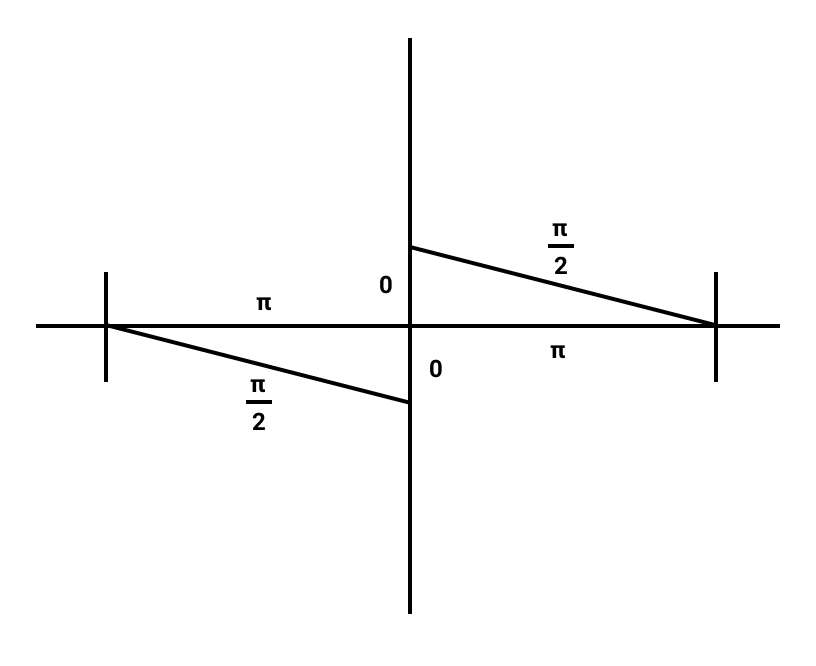
\includegraphics[width=7cm]{more_pictures/horizontal_bowtie.png}
\caption{Assignments of $\theta^*$ to edges of a bow-tie
	corresponding to an augmentation site;
	the edges labeled $\pi$ are the long edges,
	the edges labeled 0 are the short edges,
	the edges labeled $\pi/2$ are the diagonal edges}
\label{f:bowtie_angles}
\end{figure}

\begin{figure}
\begin{tabular}{cc}
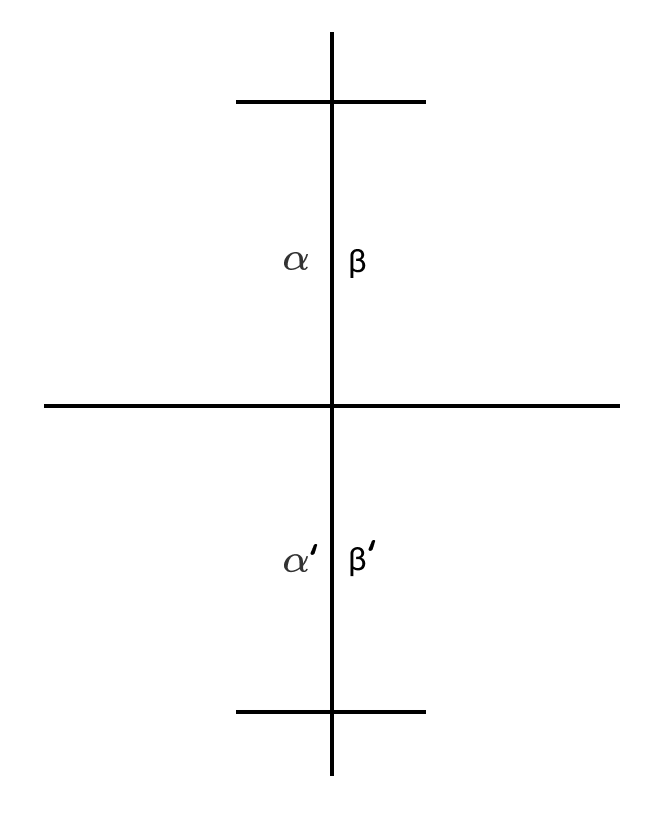
\includegraphics[width = 5cm]{before_bowtie_angles.png}&
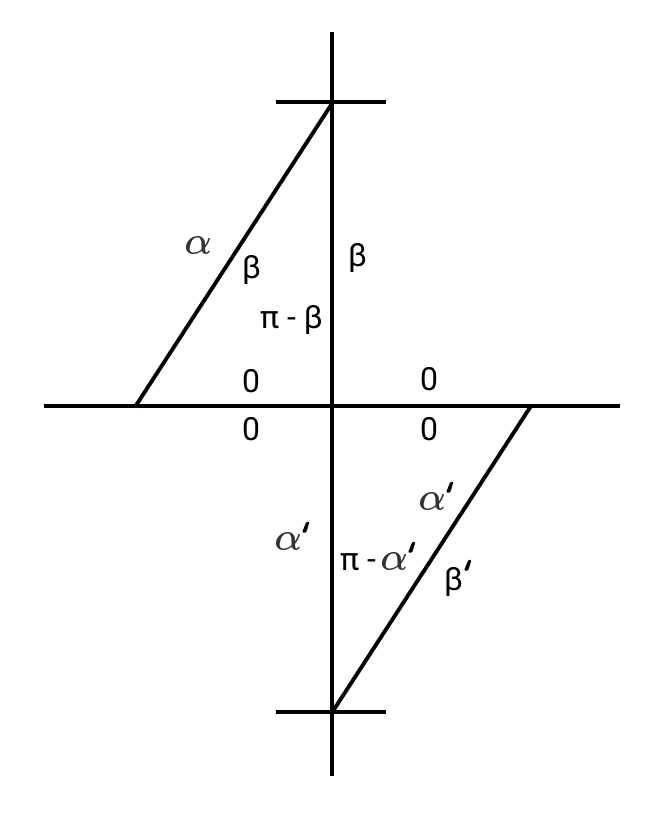
\includegraphics[width = 5cm]{bowtie_angles.png}\\
(a)&(b)
\end{tabular}
\caption{(a) Angle splitting before augmentation (b) Angle splitting for bowtie corresponding to augmentation}
\label{f:bowtie_angles2}
\end{figure}

We check that upon gluing the top and bottom torihedra,
the sum of interior dihedral angles $\theta^*$
around each edge is $2\pi$:
crossing edges have $\theta^* = \pi/2$,
and appear four times, twice in each torihedron,
while for bow-tie edges,
simply check for half-twist and non-half-twist cases
separately.


Now we have a decomposition of the two torihedra into
degenerate base-angled pyramids
(recall that that means some of the
interior dihedral angles $\theta^*$ are 0);
since we need the pyramids to be non-degenerate,
we modify the graph on the torihedra
and the angle assignments to make all $\theta^*$ nonzero
as follows.


We first modify the graphs on the torihedra by adding edges
to them for some extra ``flexibility''.
Consider a face $f$ of $\Gamma_T(L)$ that is not from a bow-tie.
Suppose the corresponding face $\bar{f}$ of $D'$
had vertices $v_1,\ldots,v_n$ in counter-clockwise order.
Note that $f$ may meet a vertex twice,
but we label each occurence with its own index.
We label the edges of $f$ by $e_{i,0}$, $e_{i,\pi}$, or $e_i$,
depending on whether the $\theta^*$ of that edge
is $0$, $\pi$, or $\pi/2$ respectively.
%with $i$ non-decreasing from 1 to $n$,
%so that adjacent edges having the same $i$ if and only if they
%belong to the same bow-tie.
More precisely, for a vertex $v_i$ corresponding to a crossing
of $K$ that is not augmented,
we label $e_{v_i}^{(.)}$ by $e_i$
(here $e_{v_i}^{(.)}$ is $e_{v_i}^{(1)}$ or $e_{v_i}^{(2)}$,
whichever meets $\bar{f}$; see \defref{d:tori-decomp-graph}).
For a vertex $v_i$ that corresponds to a twist region of $K$,
if the direction of the twist region is towards $\bar{f}$,
then $f$ meets a diagonal edge of the bow-tie corresponding to $v_i$,
and we label it $e_i$;
if not, then $f$ meets a short and long edge of the corresponding bow-tie,
and we label them by $e_{i,0}$ and $e_{i,\pi}$,
respectively.


If $\bar{f}$ does not have vertices of the latter kind,
i.e. if $f$ does not meet short or long edges,
then we will not modify $f$.
So assume that $\bar{f}$ does have such a vertex,
and suppose it is right-augmented
(the other case is treated similarly).
Then for all right-augmented vertices $v_i$ of $\bar{f}$,
$f$ would meet the short,long edges $e_{i,0},e_{i,\pi}$,
while for all left-augmented vertices,
$f$ would meet the diagonal edges.
In particular,
the edges $e_{i,0}, e_{i,\pi}$ always appear in counter-clockwise order.


Suppose, after cyclically reindexing, $v_1,\ldots,v_k$
is a maximally contiguous subsequence of right-augmented vertices
of $D'$ around $\bar{f}$;
the edges around $f$ would start
$e_{1,0} \cm e_{1,\pi} \cm e_{2,0} \cm e_{2,\pi} \cm \ldots
	\cm e_{k,0} \cm e_{k,\pi} \cm \ldots$.
We add new edges across $f$ as follows
(see \figref{f:adding_edges};
ignore the + and - signs for now.):


\begin{itemize}
\item \textbf{Case $k=n$:} (i.e. every vertex of $\bar{f}$ is right-augmented.)
In this case, we do nothing.

\item \textbf{Case: There is only one such maximal contiguous subsequence:}


\textbf{Subcase: $k=1$:}
We add an edge that goes across $e_{1,0},e_{1,\pi},e_2$
(in the sense that the new edge separates the edges of $f$ into two sets,
one of them being those three edges;
since $n\geq 3$, this edge is new).
%If $k = 2$, we add edge across $e_{1,0},e_{1,\pi}$
%and another edge across $e_{2,0},e_{2,\pi}$
%(these two edges do not form a bigon because we've ruled out $k=n$).
%(these two edges do not form a bigon because we've ruled out $k=n$).

\textbf{Subcase: $k \geq 2$:}
We add an edge across $e_{1,0},e_{1,\pi}$
and another edge across $e_{2,0},e_{2,\pi},e_{3,0},\ldots,e_{k,\pi}$
(these two edges do not form a bigon because we've ruled out $k=n$).
%(again these two edges do not form a bigon).

\textbf{Case: There are multiple such maximal contiguous subsequences.}
We just add edges as in the previous case for each contiguous subsequence,
except one special case: when the edges of $f$ are exactly
$e_{1,0},e_{1,\pi},e_2,e_{3,0},e_{3,\pi},e_4$,
we add only one edge separating the first three edges from the other three.
(This prevents formation of a bigon.)
\end{itemize}


\begin{figure}
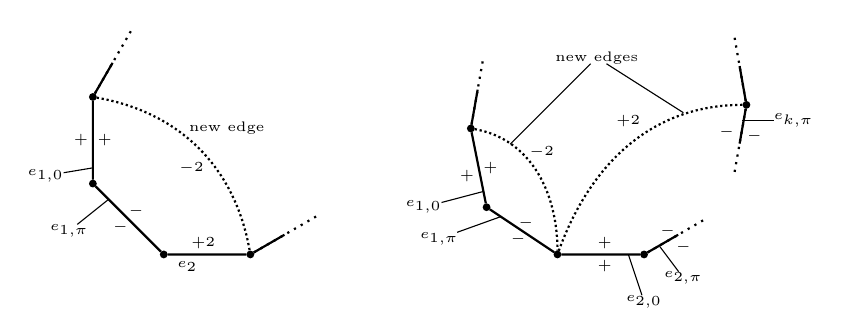
\begin{tikzpicture}
\begin{scope}[shift={(0,0)}]
\node[dotnode] (a) at (-1,2) {};
\node[dotnode] (b) at (-1,0.9) {};
\node[dotnode] (c) at (-0.1,0) {};
\node[dotnode] (d) at (1,0) {};
\draw (a) -- (b) -- (c) -- (d);
\draw[dotted] (a) -- +(60:1cm);
\draw (a) -- +(60:0.5cm);
\draw[dotted] (d) -- +(30:1cm);
\draw (d) -- +(30:0.5cm);
\draw[densely dotted] (a) to[out=-10,in=100] (d);
%% labels, edge by edge
\node[inner sep=0, outer sep=0] (e10) at (-1.6,1.0) {\tiny $e_{1,0}$};
\draw[line width=0.4pt] (e10) -- (-1,1.1);
\node at (-1.15,1.45) {\tiny $+$};
\node at (-0.85,1.45) {\tiny $+$};
%%
\node[inner sep=0, outer sep=0] (e1pi) at (-1.3,0.3) {\tiny $e_{1,\pi}$};
\draw[line width=0.4pt] (e1pi) -- (-0.8,0.7);
\node at (-0.65,0.35) {\tiny $-$};
\node at (-0.45,0.55) {\tiny $-$};
%%
\node at (0.2,-0.15) {\tiny $e_2$};
\node at (0.4,0.15) {\tiny $+2$};
%%
\node at (0.7,1.6) {\tiny new edge};
\node at (0.25,1.1) {\tiny $-2$};
\end{scope}
%%%%%%%%%%%%%%%%%%%%%%%%%%%%%%%%%%%%%%%%%%%%%%
\begin{scope}[shift={(5,0)}]
\node[dotnode] (e) at (-1.2,1.6) {};
\node[dotnode] (a) at (-1,0.6) {};
\node[dotnode] (b) at (-0.1,0) {};
\node[dotnode] (c) at (1,0) {};
\node[dotnode] (d) at (2.3,1.9) {};
\draw (e) -- (a) -- (b) -- (c);
\draw[dotted] (e) -- +(80:0.9cm);
\draw (e) -- +(80:0.5cm);
\draw[dotted] (c) -- +(30:0.9cm);
\draw (c) -- +(30:0.5cm);
\draw[dotted] (d) -- +(-100:0.9cm);
\draw (d) -- +(-100:0.5cm);
\draw[dotted] (d) -- +(100:0.9cm);
\draw (d) -- +(100:0.5cm);
\draw[densely dotted] (e) to[out=-10,in=90] (b);
\draw[densely dotted] (b) to[out=70,in=180] (d);
%% labels
\node[inner sep=0, outer sep=0] (e10) at (-1.8,0.6) {\tiny $e_{1,0}$};
\draw[line width=0.4pt] (e10) -- (-1.04,0.8);
\node at (-1.25,1.0) {\tiny $+$};
\node at (-0.95,1.1) {\tiny $+$};
%%
\node[inner sep=0, outer sep=0] (e1pi) at (-1.6,0.2) {\tiny $e_{1,\pi}$};
\draw[line width=0.4pt] (e1pi) -- (-0.82,0.48);
\node at (-0.5,0.4) {\tiny $-$};
\node at (-0.6,0.2) {\tiny $-$};
%%
\node[inner sep=0, outer sep=0] (e20) at (1,-0.6) {\tiny $e_{2,0}$};
\draw[line width=0.4pt] (e20) -- (0.8,0);
\node at (0.5,-0.15) {\tiny $+$};
\node at (0.5,0.15) {\tiny $+$};
%%
\node[inner sep=0, outer sep=0] (e2pi) at (1.5,-0.3) {\tiny $e_{2,\pi}$};
\draw[line width=0.4pt] (e2pi) -- (1.2,0.1);
\node at (1.3,0.3) {\tiny $-$};
\node at (1.5,0.1) {\tiny $-$};
%%
\node[inner sep=0, outer sep=0] (ekpi) at (2.9,1.7) {\tiny $e_{k,\pi}$};
\draw[line width=0.4pt] (ekpi) -- (2.25,1.7);
\node at (2.4,1.5) {\tiny $-$};
\node at (2.05,1.55) {\tiny $-$};
%%
\node at (-0.3,1.3) {\tiny $-2$};
\node at (0.8,1.7) {\tiny $+2$};
%%
\node[inner sep=0, outer sep=0] (n) at (0.4,2.5) {\tiny new edges};
\draw[line width=0.4pt] (n) -- (-0.7,1.4);
\draw[line width=0.4pt] (n) -- (1.5,1.8);
\end{scope}
\end{tikzpicture}



\caption{Adding edges to non-bow-tie faces;
the $+/-$ labels are short for $+1/-1$.}
%edge indicates an added edge to $\Gamma_T(L)$;
%indicate whether to
%increase/decrease $\vphi$ (and $\theta^*$)
\label{f:adding_edges}
\end{figure}


This way we obtain a new graph $\Gamma_T'$, which defines a
new torihedron $\sT_T'$.
We make $\sT_T'$ angled using the angles from $\sT_T(L)$ for old edges,
and putting $\theta^* = \pi$ for all new edges.


We can get an angle-splitting for $(\Gamma_T',\theta^*)$,
using the angle-splitting for $\Gamma_T(L)$ for old edges,
and for a new edge $e$ that cuts through some face $f$ of $\Gamma_T(L)$,
we assign $\vphi_{\vec{e}} = \sum \vphi_{\vec{e'}}$,
where the sum is over all the edges $\vec{e'} \in \del f$
that on the other side of $\vec{e}$.
It is easy to see that the new assignments are all non-zero
(follows from non-degeneracy of the angle-splitting on $D'$).


Now fix some small $\veps > 0$.
Let $\vphi_{\vec{e}}' = \vphi_{\vec{e}} + x \cdot \veps$,
where $x$ is the label on $\vec{e}$ (0 if unlabeled).
Let $\theta_e'^* = \vphi_{\vec{e}}' + \vphi_{\cev{e}}'$.
It is easy to check that the sum of $\theta'^*$
around each vertex is the same as for $\theta^*$,
so it defines an angled torihedron $(\sT_T',\theta'^*)$.
For each face of $\Gamma_T'$, the $+/-$ labels
on the inner side of boundary edges cancel out:
for bow-tie faces, the short edge gets a $+1$ and the long edge
gets $-1$, while for non-bow-tie faces,
it is clear from \figref{f:adding_edges}.
Hence, $\vphi'$ is an angle-splitting of $(\sT_T',\theta'^*)$.
Furthermore, all shorts edges
(which are the only edges with $\vphi_{\vec{e}} = 0$)
have a $+1$ label on each side,
so $\vphi'$ is non-degenerate.


Now we perform the same operations for the bottom torihedron,
adding new edges to $\Gamma_B(L)$ to get $\Gamma_B'$
in the same manner;
note that left and right augmentations are switched,
so that the order of $e_{i,0},e_{i,\pi}$ are switched.
Thus all the $+/-$ labels in \figref{f:adding_edges}
should have switched signs.
We also get a nondegerate angle-splitting $\vphi'$
of an angled torihedron $(\sT_B',\theta'^*)$.


By construction, under the gluing of
$\sT_T(L)$ to $\sT_B(L)$,
the new edges added to $\Gamma_T(L)$
are glued to the new edges added to $\Gamma_B(L)$,
since they are added by the same procedure.
As noted before, upon gluing $\sT_T(L)$ to $\sT_B(L)$
the sum of exterior dihedral angles $\theta^*$ around each edge
is $2\pi$.
This clearly remains true after adding the new edges
(they're label $\pi$ on each torihedron).
Again by construction,
the $+/-$ labels coming from the top and bottom diagrams get canceled out.
Thus, upon gluing $\sT_T'$ to $\sT_B'$,
the sum of new exterior dihedral angles $\theta'^*$ around each edge
is $2\pi$.


Finally, we obtain a triangulation with an angle structure as follows.
For each face of $\Gamma_T'$ that has more than three sides,
we arbitrarily decompose it into triangles
and apply \lemref{l:pyramid_decomp}
to obtain a triangulation of $\sT_T'$ into non-degenerate angled tetrahedra;
perform the corresponding decomposition for faces of
$\Gamma_B'$ and obtain a triangulation of $\sT_B'$
into non-degenerate angled tetrahedra.
These triangulations glue up into a triangulation of $\toruscomp{L}$
with an angle structure.
Thus, $L$ is hyperbolic.
\end{proof}


\bibliographystyle{plain}
\bibliography{references-ak}

%%% comment }

\end{document}


%%Figures for easy look up

%augmenting twist regions
%\label{fig:Augmentations}

%left right augmentations
%\label{f:right_left_aug}

%crossing edge, Menasco thing
%\label{fig:crossingArc} 
%\label{f:crossing-edges}.

%cut-slice-flatten, bow-ties, gluing
%\label{fig:falGluings}

%definition of the torihedral decomp graph
%\label{d:tori-decomp-graph}

%assignments of theta^*
%\label{f:bowtie_angles}

%assigment of +/- labels
%\label{f:adding_edges}
